%--------------------
% Packages
% -------------------
\documentclass[11pt,a4paper]{article}
\usepackage[utf8x]{inputenc}
\usepackage[T1]{fontenc}
%\usepackage{gentium}
%\usepackage{mathptmx} % Use Times Font
\usepackage{url}
%\usepackage{natbib}
%\usepackage{biblatex}
%\setlength\bibitemsep{\baselineskip}
\usepackage[english]{babel}
%Includes "References" in the table of contents
\usepackage[nottoc]{tocbibind}
\usepackage{multicol}
\usepackage{mathtools}
\usepackage{natbib}
\setlength{\bibsep}{0pt plus 0.0ex}


\usepackage[pdftex]{graphicx} % Required for including pictures
\usepackage{subcaption}
\usepackage[export]{adjustbox}
\usepackage[pdftex,linkcolor=black,pdfborder={0 0 0}]{hyperref} % Format links for pdf
\usepackage{calc} % To reset the counter in the document after title page
\usepackage{enumitem} % Includes lists
\usepackage{xcolor}
\usepackage{soul}
\captionsetup[figure]{font=small,labelfont=small}
\usepackage{etoolbox}
\usepackage{titlesec}
\titlespacing*{\section}{0pt}{0.1\baselineskip}{0.2\baselineskip}
\titlespacing*{\subsection}{0pt}{0.3\baselineskip}{0.4\baselineskip}

\frenchspacing % No double spacing between sentences
\linespread{1.05} % Set linespace
\usepackage[a4paper, lmargin=2cm, rmargin=2cm, tmargin=2cm, bmargin=2cm]{geometry} %margins


\usepackage[all]{nowidow} % Tries to remove widows
\usepackage[protrusion=true,expansion=true]{microtype} % Improves typography, load after fontpackage is selected

\usepackage{lipsum} % Used for inserting dummy 'Lorem ipsum' text into the template

%-----------------------
% Begin document
%-----------------------
\begin{document}
\AtBeginEnvironment{thebibliography}{\fontsize{9}{\baselineskip}\selectfont}

\onecolumn

\begin{center}
\textbf{\fontsize{18}{\baselineskip}\selectfont The effect of microstructure, porosity, and graphite content on the cyclic fatigue properties of cast iron from the 19th century}
\bigskip

\fontsize{14}{\baselineskip}\selectfont Kyprianos Kythreotis

\bigskip
\bigskip
\bigskip
\bigskip
\end{center}

\noindent \textbf{\fontsize{14}{\baselineskip}\selectfont Summary}

\bigskip

\noindent The objective of this research project is to develop a computational toolbox that can assess the remaining life of grey cast iron components extracted from any UK infrastructure structure. Grey cast iron has been used since the 19th century due to its low cost, reliability, and durability. However, these structures can become fatigued over time and compromise safety. Therefore, the study examines the impact of micro-structural features, including pores, graphite content, and surface roughness, on the cyclic fatigue life of grey cast iron. By using modern modelling techniques, small-scale testing, and microscopy characterization, the project aims to develop a multi-scale model that can predict the lifetime of grey cast iron components under different loading conditions and micro-structural variations with high accuracy. In more detail, the work involves cyclic fatigue experiments, optical and scanning electron microscopy, and phase field fracture modelling. The results of the experiments showed that the specimen from the Clifton Suspension bridge stanchion part, fractured significantly earlier than previously conducted experiments, on grey cast iron specimens that was researched in literature. This lead to the microscopy imaging of the specimen, which analysis revealed an accumulation of graphite on the fractured surface and the presence of porosity with a suggested estimated pore size range. Afterwards the phase field fracture model was extended to account for cyclic loading and was calibrated to match the researched experimental literature results. Then, the features were incorporated into the model as well, where the pore specimen model simulations matched the experimental results of this work. Also, the model specimen including the pore or graphite flake, demonstrated a decrease of its fatigue life for both, when compared to the model simulation without any features. The reduction of the fatigue life of the specimen including different size pore or graphite flake was recorded, and showed a relationship. It was concluded therefore that porosity had a much higher negative effect than graphite on the reduction of the fatigue life. Also, the computational toolbox to accurately predict the lifetime of grey cast iron components at different length scales, accounting for micro-structural variations, and loading conditions, was created and tested. The multi-scale model can be implemented for any grey cast iron component that is used in existing infrastructure. The main limitation associated with the model created is that it considers only constant amplitude cyclic loading and so, further research could include the investigation of more complex loading regimes.

\bigskip

\bigskip

\bigskip

\bigskip

\begin{center}
\fontsize{14}{\baselineskip}\selectfont  Supervised by Dr. Nicolò Grilli

\bigskip

\fontsize{14}{\baselineskip}\selectfont Department of Mechanical Engineering

\bigskip

\fontsize{14}{\baselineskip}\selectfont University of Bristol

\bigskip

\fontsize{14}{\baselineskip}\selectfont 2023

\end{center}
\bigskip
\bigskip
\bigskip
\bigskip
\bigskip
\bigskip
\bigskip
\bigskip
\bigskip
\bigskip
\bigskip
\bigskip
\bigskip
\bigskip
\bigskip
\bigskip
\bigskip
\bigskip
\bigskip
\bigskip
\bigskip
\bigskip
\bigskip
\bigskip
\bigskip
\bigskip
\bigskip
\bigskip
\bigskip
\bigskip
\bigskip
\bigskip
\bigskip
\bigskip
\bigskip
\bigskip
\bigskip
\bigskip
\bigskip
\bigskip
\bigskip
\bigskip
\bigskip
\bigskip
\bigskip
\bigskip
\bigskip
\bigskip
\bigskip
\begin{center}
\textbf{\fontsize{16}{\baselineskip}\selectfont Declaration}

\bigskip

This project report is submitted towards an application for a degree in Mechanical Engineering at the University of Bristol. The report is based upon independent work by the candidate. All contributions from others have been acknowledged and the supervisor is identified on the front page. The views expressed within the report are those of the author and not of the University of Bristol.
I hereby assert my right to be identified as the author of this report. I give permission to the University of Bristol Library to add this report to its stock and to make it available for consultation in the library, and for inter-library lending for use in another library. It may be copied in full or in part for any bona fide library or research worker on the understanding that users are made aware of their obligations under copyright legislation.
I hereby declare that the above statements are true.
{Student signature}
\bigskip
\bigskip
\bigskip
\bigskip
\bigskip
\bigskip
\bigskip
\bigskip
\bigskip
\bigskip
\bigskip


© Copyright, {student name, year}
Certification of ownership of the copyright in a dissertation presented as part of and in accordance with the requirements for a degree in Mechanical Engineering at the University of Bristol.
This report is the property of the University of Bristol Library and may only be used with due regard to the author. Bibliographical references may be noted but no part may be copied for use or quotation in any published work without prior permission of the author. In addition, due acknowledgement for any use must be made.
\end{center}
\bigskip
\bigskip
\bigskip
\bigskip
\bigskip
\bigskip
\bigskip
\bigskip
\bigskip
\bigskip
\bigskip
\bigskip
\bigskip
\bigskip
\bigskip
\bigskip
\bigskip
\bigskip
\bigskip
\bigskip
\bigskip
\bigskip
\bigskip
\bigskip
\bigskip
\bigskip
\bigskip
\bigskip
\bigskip
\bigskip
\bigskip
\bigskip
\bigskip

\tableofcontents


\bigskip
\bigskip
\bigskip
\bigskip
\bigskip
\bigskip
\bigskip


\section{Introduction}

Civil engineering has fulfilled a crucial role in shaping the modern world by providing the infrastructure and facilities that enable the functioning of modern societies. The motivation of the project lies in the need to assess the safety and remaining life of these structures, particularly those made of grey cast iron, to improve their safety, save money, and reduce emissions.

\noindent Grey cast iron has been used extensively in the UK and worldwide infrastructure since the 19th century, because it is cheap, easy to make, reliable, has a long lifetime, and is resistant to atmospheric agents. In the UK, cast iron has been widely used for constructing bridges, buildings, and sewage systems during the Industrial Revolution. According to a study by the British Cast Iron Research Association, more than 5000 cast iron bridges were built in the UK between 1796 and 1930 \cite{doi:10.1680/jenhh.17.00005}. Cast iron was also commonly used for water supply systems, including pipes, valves, and hydrants \cite{cosham2001durability}. Worldwide, cast iron has been used in a variety of infrastructure applications, such as pipelines, water treatment plants, and transportation systems. For example, in the United States, cast iron pipes were widely used for water distribution systems until the mid-20th century, with an estimated 6 million miles of cast iron pipes installed by the 1950s \cite{snider2021preparing}.

\noindent As it is known for its features mentioned above, it is an attractive option for many engineering applications. However, these structures are still in use today and are subject to fatigue and deterioration, which can compromise their safety and structural integrity. The components of such old infrastructures were not produced in series and most of them are custom made. There is substantial difference between all component dimensions and materials, introducing variability in the material. This was caused as there was no standardization on the casting. Therefore, it is essential to evaluate their remaining life to ensure public safety and avoid catastrophic failures.

\noindent This assessment though could be extremely expensive as large-scale testing would require a lot of computational power and equipment for the experiments. Therefore, in this work, it is proposed to use a combination of modern modelling techniques, small scale testing, and microscopy characterization, which were not available in the past, thus improving the accuracy of the prediction. Small-scale testing of grey cast iron can provide insights into the microstructure and defects that affect its fatigue behavior, which can be used to predict its behavior in larger structures. Also, it provides a representative sample of the material's properties, as it allows for a controlled environment and eliminates the variability that can be present in large-scale testing. Moreover, since the techniques include micro-structural features like pores, and graphite, they can assess a large variety of components.

\noindent The vision is to develop a multi-scale strategy that can use the micro-scale information to calibrate models that can be applied at all length scales. This will be achieved by length scale sensitive phase field modelling techniques that can be applied to different length scales based on a single microscopic calibration. In this project such approach is demonstrated on samples extracted from the stanchion part of the Clifton Suspension bridge. However, the results of this project have shown that such methodology can be applied to all UK infrastructure structures built from cast iron.

\section{Literature Review}
\subsection{Grey cast iron cyclic fatigue}
Grey cast iron is a widely researched material due to its applications in the production of the automotive components. The fatigue life of grey cast iron is assessed through a completely reversed load control axial loading fatigue test \cite{fash1982fatigue}. The classification of the free graphite structure size and distribution is given by ASTM standard A2475 as approximately 60\% type A, and approximately 40\% type D. Type A translates to the fact that the graphite structure is characterized by relatively small flakes that are uniformly distributed in the metal matrix, and type D, to the fact that the graphite structure is characterized by larger, more irregular flakes that are often clustered together \cite{ASTM:A247}. The results of the work are presented in figure \ref{S_N}, where it shows the maximum applied stress amplitude against the number of cycles to failure (S-N graph). The S-N graphs are parameterised using stress-based parameters, such as stress amplitude or stress range. This is because brittle materials, such as cast iron, fail due to the initiation and growth of cracks under cyclic loading conditions, and the stress-based parameters are more appropriate for characterizing crack initiation and growth. Moreover, an axial loading fatigue test on flake graphite cast iron specimens, where the experiment was stopped if it reached $10^7$ cycles, was performed \cite{shirato2018study}. According to the classification of graphite in cast iron, it was categorized as Distribution A Graphite in isotropic material \cite{ASTM:A247}. This distribution indicates that the graphite flakes are evenly distributed throughout the material, with no clustering or agglomeration. The results are also shown in figure \ref{S_N}. The researched literature data are analysed to be compared with the experimental data of this work.
\subsection{Porosity effect on fatigue life}
Pores are cavities or empty spaces that form in the solidification process within a casting. Porosity in general, is caused by three sources: macro shrinkage, microporosity, and gas porosity. A casting design that inhibits appropriate feeding can cause macro shrinkage, which includes large deficiencies, like misruns and cold shuts \cite{boileau2001effect}. Gas porosity happens when bubbles of gas are formed in the material in a spherical or irregular shape \cite{Frant}. Minimal amount of work was executed regarding the porosity effect on grey cast iron because complex microscopy techniques are needed, which were not available in the past. Instead, studies performed on similar cast materials were researched. Firstly, fatigue fractured small cylindrical ductile cast iron (DCI) specimens demonstrated that especially in the porosity areas, porosity was the primary cause of fracture under high-cycle fatigue \cite{https://doi.org/10.1111/ffe.13783}. This was showed after the specimens were subjected to both uniaxial (tension or torsion) and biaxial (combined compression and torsion) cyclic loading with a constant amplitude. In addition, pores were observed to act like the major sites of the fatigue crack nucleation along with accelerating the process, if observed near the surface \cite{kainzinger2013influence}. Furthermore, porosity in cast aluminium alloys has a crucial effect on its fatigue life. After uniaxial fatigue tests were performed at room temperature with a frequency of 40 Hz and a stress ratio R of -1, it was determined that porosity decreases time to the initiation of the crack as it creates a concentration of high stress in the material \cite{boileau2001effect}. Lastly, axial fatigue testing on cast steel specimens concluded that porosity causes large stress concentrations on the area of the pores, and therefore decreases their fatigue life \cite{prediction}. Consequently, it could be understood that for all materials researched for, porosity has a negative effect on the fatigue life of the material specimens. Therefore, the aim related to this aspect of the project, is to examine the grey cast iron response in respect to the pore size it contains, and how that affects its life. Crack initiation and propagation on the surface of the specimen due to porosity is also examined and evaluated.
\subsection{Graphite effect on fatigue life}
Grey cast iron specimens contain graphite flakes which serve as stress concentration points, making the material more brittle and prone to cracking. Through fatigue testing, evidence suggested that cracks were formed at the tips of the flakes that were positioned perpendicular to the maximum principal stress, on the surface of the specimen. Moreover, cracks propagate from flake to flake in a direction that is normal to the maximum principal stress \cite{WEINACHT198779}. It was also showed that the specimen that contains the higher fraction of graphite, will result with the lower fatigue strength \cite{yilagaqi2023effect}. However, it was identified that the fatigue behaviour is mostly influenced by the porosity present on the surface, than the fraction of graphite content \cite{borsato2016mechanical}. The pursue of the project relating to the graphite fraction, consists of examining the response of graphite on the non-fractured and fractured specimen. Also, the effect of different graphite flake sizes on the fatigue life of the grey cast iron specimens is investigated.
\subsection{Phase field fracture modeling}
Phase field fracture is a mathematical approach that replaces sharp crack surfaces with diffusive zones, gradually degrading the material from intact to fully broken, making it a useful tool for fracture mechanics modeling and simulation \cite{miehe2010phase}. At the microscopic scale, the phase field fracture model can be used to simulate fracture behavior in small specimens and predict the crack's path and fracture toughness of the material. This information can then be used to design and optimize the performance of the material or structure. At the macroscopic scale, the phase field fracture model can be applied to larger structures, such as bridges, to predict the overall failure behavior and identify potential failure points. The phase field fracture model offers several advantages over other fracture models. For example, it can handle complex fracture patterns, such as crack branching and merging, and can predict the evolution of the crack surface in real time. It also provides a continuous representation of the crack surface, which can be useful for predicting the mechanical behavior of the material or structure in the presence of cracks \cite{miehe2010phase} \cite{kristensen2016assessment}. In this work, the base phase field fracture model is extended to cyclic loading. The base method is not suitable for it, because the strain energy depends only on the monotonic application. This implies that complex work is needed for the extension to occur.

\section{Aims and Objectives}
\label{sec:objectives}

\subsection{Aims}

The primary aim of this research project is to investigate the impact of micro-structural features, such as pores, graphite content, and surface roughness on the cyclic fatigue life of grey cast iron. The project also aims to develop a multi-scale model that can accurately predict the lifetime of grey cast iron components at different length scales, accounting for micro-structural variations, and loading conditions. To achieve these, a combination of mechanical testing and optical and scanning electron microscopy, will be utilized to validate the developed model and ensure its reliability under various micro-structural configurations. The project's goal is to assess the durability and advance the sustainability of cast iron structures, contributing to the development of more sustainable infrastructure while preserving cultural heritage for future generations.

\subsection{Objectives}

These overarching aims are achieved by the following objectives:
\vspace{-2mm}
\begin{enumerate}
\setlength\itemsep{-0.2em}
\item\label{O1} Carry out cyclic fatigue testing of grey cast iron specimens extracted from Clifton Suspension bridge to measure their fatigue life
\item\label{O2} Optical microscopy characterization to assess the pore size
\item\label{O3} Electron microscopy characterization to assess the fracture surface and possible origin of fatigue failure, as well as the surface roughness and graphite content
\item\label{O4} Extension of phase field fracture model to the case of cyclic fatigue to result in a modified model that is informed by porosity and graphite flake content, and can be applied to a component of different length
\item\label{O5} Implementing the model in a finite element solver
\item\label{O6} Calibrating, verifying and validating the model to reproduce existing experiments in the literature and the experiment in this work
\item\label{O7} Using the model to understand the degradation of fatigue life due to pores and graphite flakes accumulation with different sizes and shapes
\item\label{O8} Creating a computational toolbox, linked to a FEM solver, that can be readily used to assess the reduction of the fatigue life in components with arbitrary shape and size, and in a wide range of loading conditions as a function of porosity and graphite content
\end{enumerate}

\section{Experimental Characterisation}
\subsection{Cyclic fatigue experimental set up and results}
The grey cast iron specimens were machined and prepared into the dogbone shape, as presented in figure \ref{dogbone}, after being extracted from old stanchions unmounted from the Clifton Suspension bridge. The figure also indicates the specimen's length and thickness $ \left [ \textrm{mm}  \right ]$. The constant amplitude, fully reversed, cyclic load experiment was performed on the Instron 1341 machine, where the load amplitude was alternating between a preset maximum and minimum value. This machine was specifically chosen because of its capability to perform cyclic fatigue testing on the grey cast iron specimens accurately and reliably, and for its versatility and ease of use. The testing was load-controlled and the frequency was maintained at a constant value of 50 Hz throughout the experiment to allow for the evaluation of the fatigue strength and fatigue life of the material. The cast iron specimens were cycled up to their fracture point, where the number of cycles to failure and the maximum and minimum load and displacements values were recorded for every one of them. The set up of the experiment is shown in figure \ref{machine}. After conducting the experiment for a range of stress magnitudes, a graph of maximum stress applied, against the number of cycles to failure (S-N graph), is plotted using a logarithmic x-axis and shown in figure \ref{S_N}. This clearly shows how objective \ref{O1} is achieved, where the fatigue life of the grey cast iron specimens was measured. The analysis of the S-N graph is a standard method recommended by ASTM standards to evaluate the fatigue properties of materials and determine its fatigue strength and life \cite{ASTME466-07}. The analysis is done in section \ref{S-N analysis}. By comparing the experimental data to the researched literature data, where both can be seen in figure \ref{S_N}, it is deduced that the behaviour of the researched experimental specimens, was not examined after $10^6$ or $10^7$ cycles, because to reach that high number of cycles is time consuming. In addition, the grey cast iron experimental literature specimens fractured at a higher number of cycles than the experimental data, showing a higher fatigue life, especially at the large amplitude stresses. Also, the researched flake graphite cast iron specimens, illustrated a higher fatigue strength than the experimental data of this work and the grey cast iron experimental literature data, which also consist of graphite flakes in their microstructure. These observations therefore, motivated us to investigate the micro-structural features of the samples of this work, using microscopy and finite element simulations. 

\begin{figure} [ht]
\begin{subfigure}{0.5\textwidth}
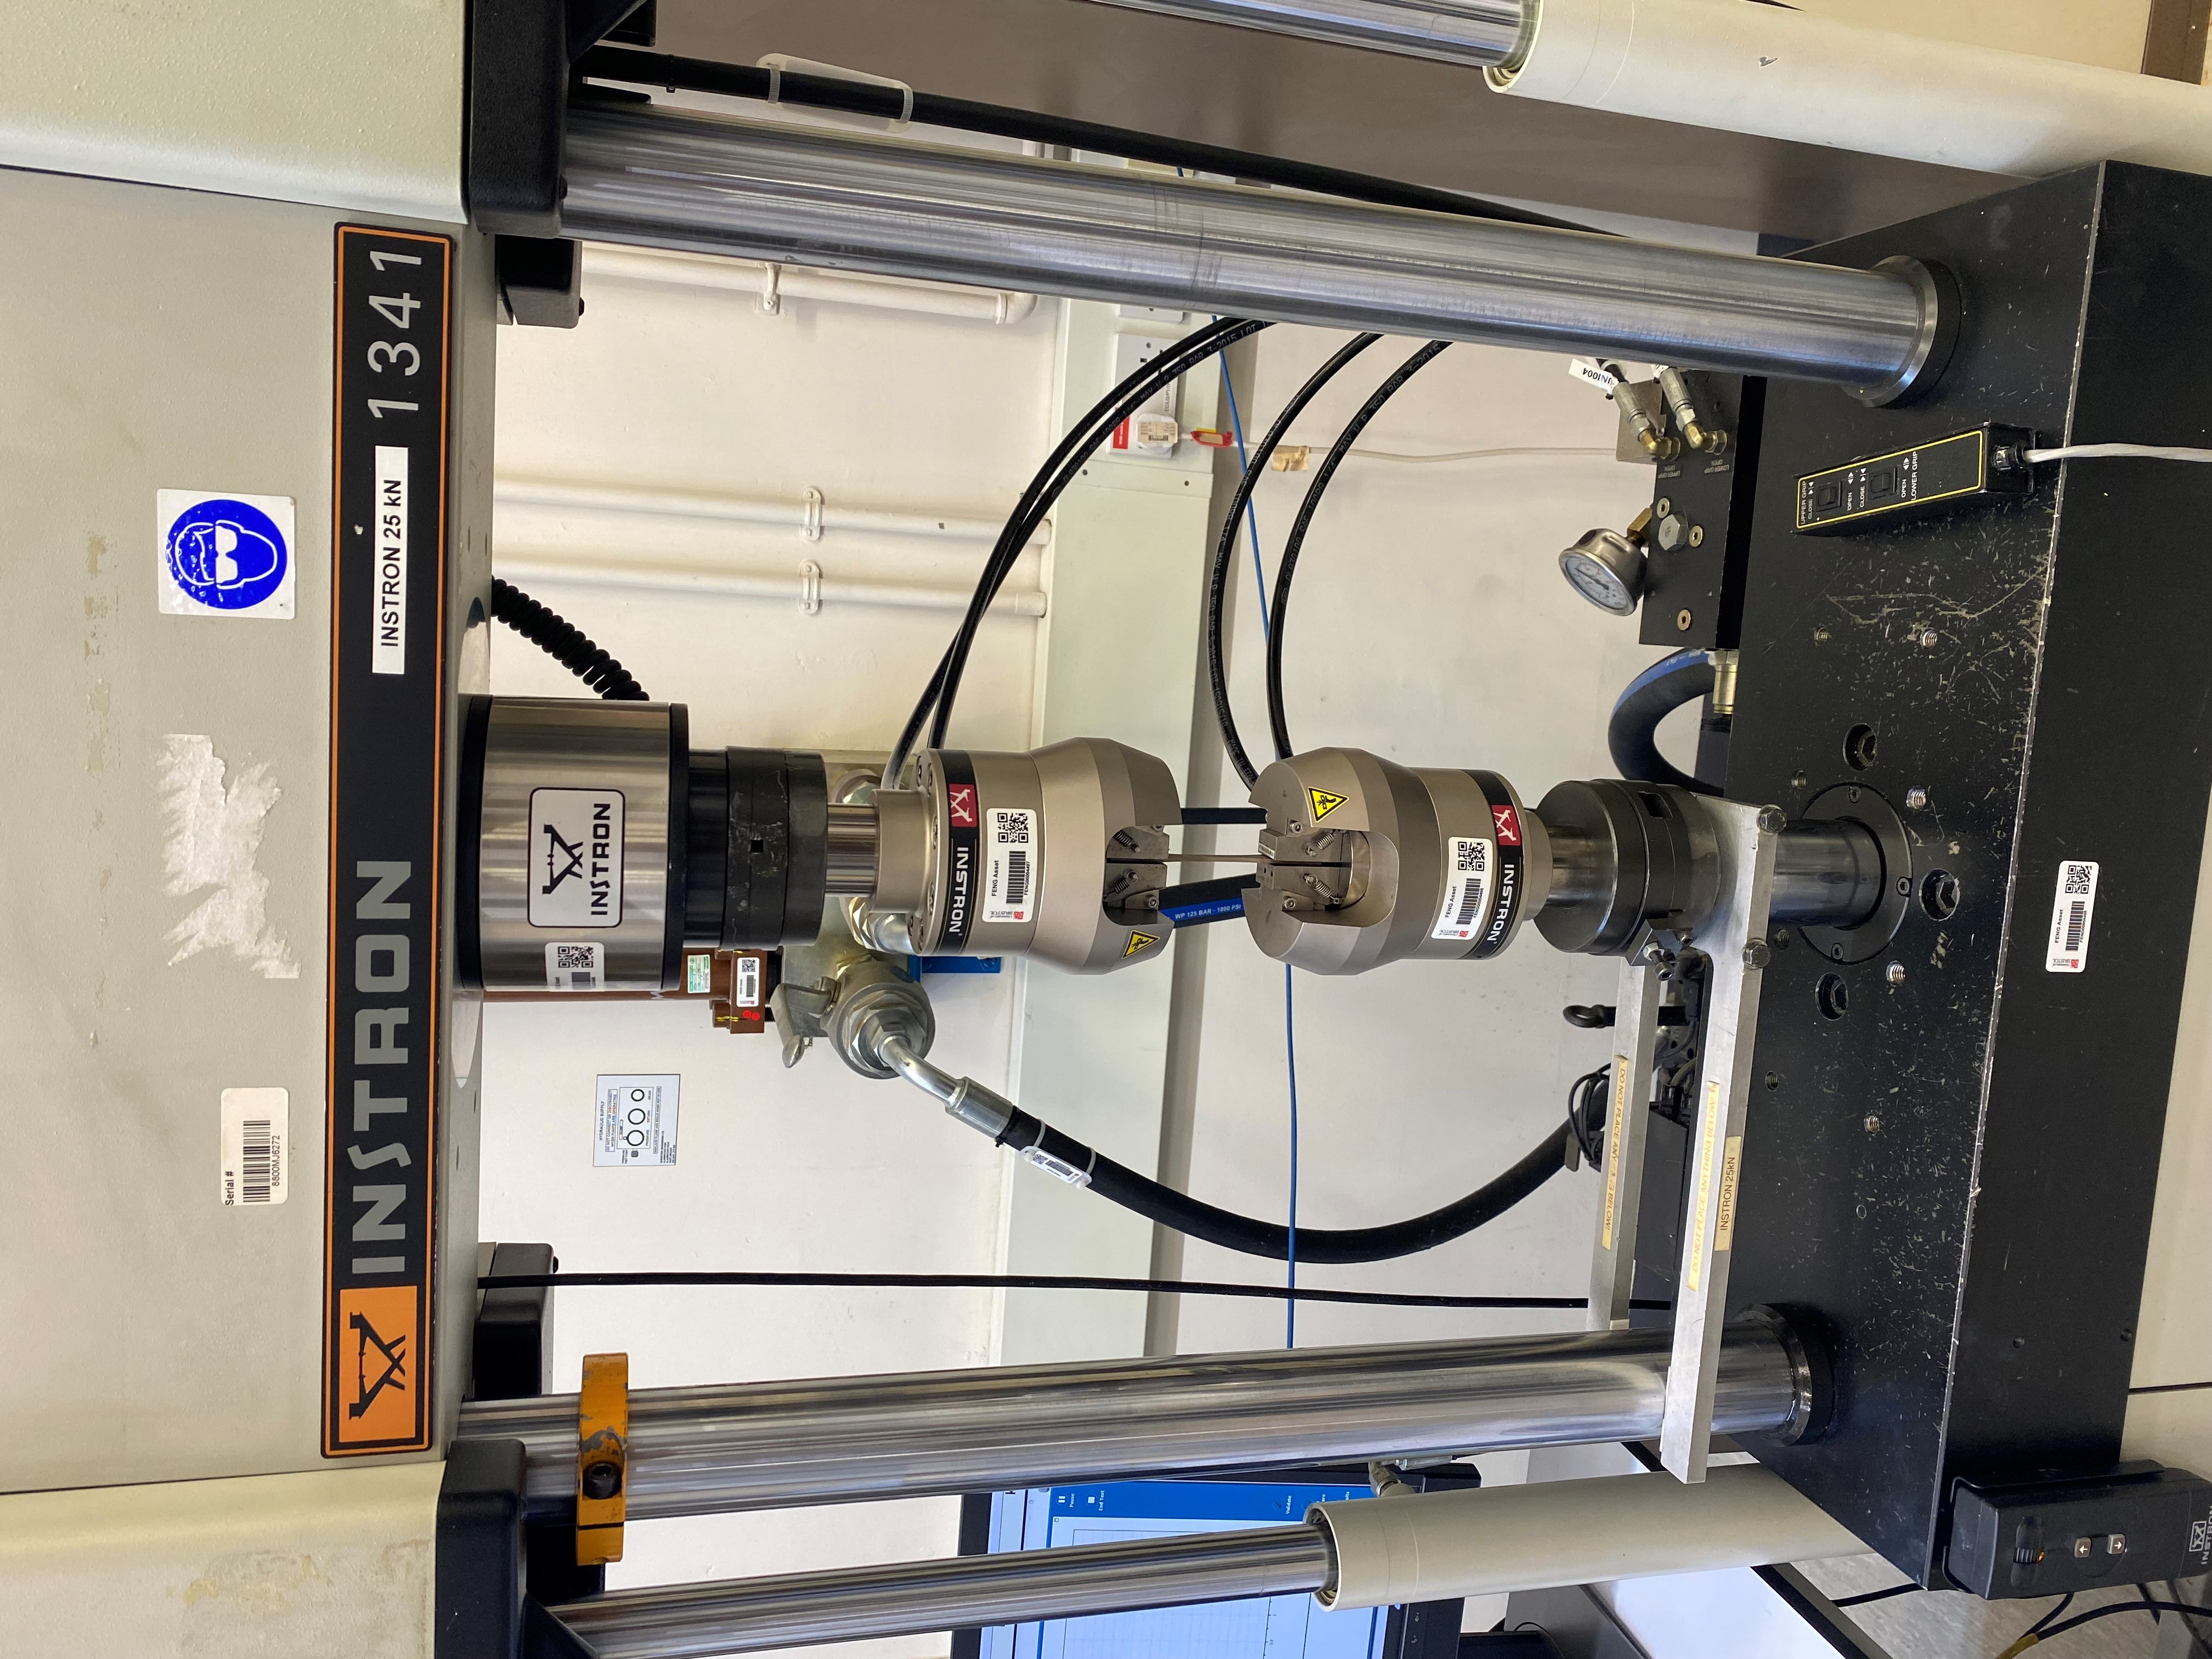
\includegraphics[scale=0.05, angle=270, center]{Instron_full.png}
\caption{Instron tensile testing machine}
\label{machine}
\end{subfigure}
\begin{subfigure}{0.5\textwidth}
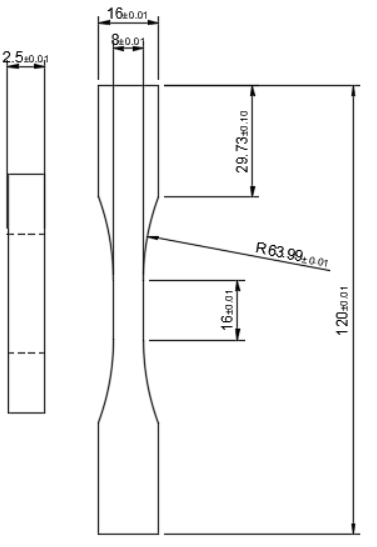
\includegraphics[scale=0.61, angle=0, center]{dogbone_specimen.png}
\caption{Dogbone specimen sketch [mm]}
\label{dogbone}
\end{subfigure}
\caption{Experimental set up and specimen size for the cyclic fatigue.} 
\end{figure}

\begin{figure} [ht]
\centering
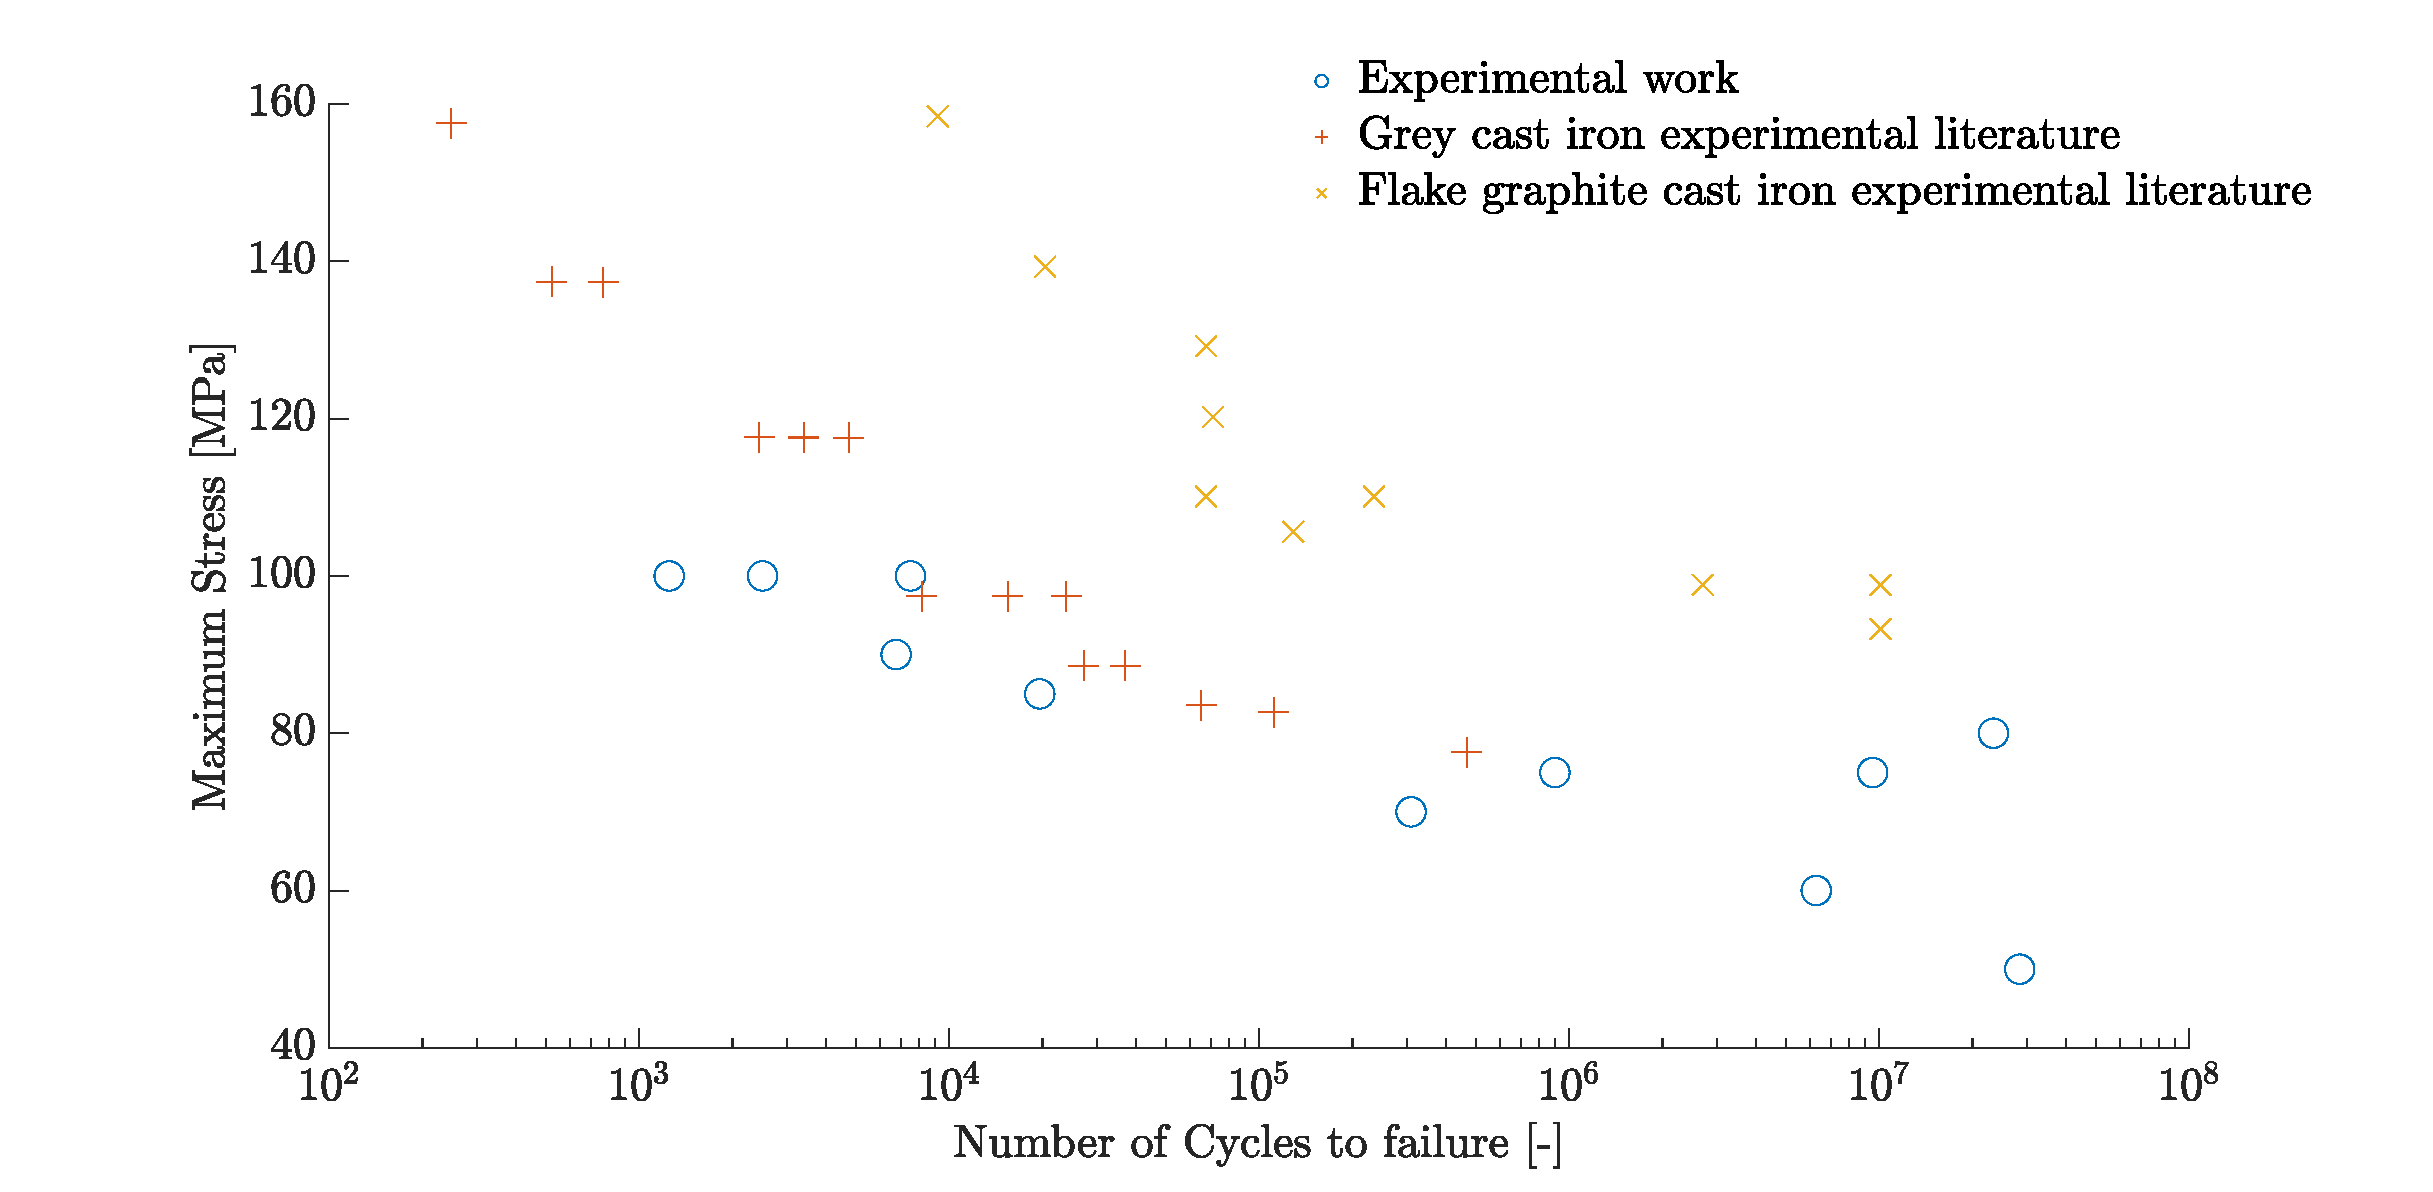
\includegraphics[width = 17cm]{S-N_curve.eps}
\caption{Maximum stress amplitude against the number of cycles to failure.}
\label{S_N}
\end{figure}

\subsection{Microscopy characterisation of grey cast iron}
Using an optical microscope, the grey cast iron surface can be examined and analyzed. Features like flake graphite and pearlite regions are identified. The specimens were polished with colloidal silica. Figure \ref{optical_side} shows the optical microscopy at multiple magnifications (10×, 20×, and 50×) \cite{de2020multi}. The results represent a 10x magnification of the specimen before and after etching with Nital 2\%, and a 50x magnification after etching. The graphite flakes are presented as black in figure \ref{optical_side}, and the pearlite regions as white in figure \ref{10_after_etching} and \ref{50_after_etching}. The information from the microscopy images about the graphite fraction of the specimen will be used in section \ref{Image_analysis} to understand the effect of graphite on the remaining life of the component.

\begin{figure} [ht]
\begin{subfigure}{0.335\textwidth}
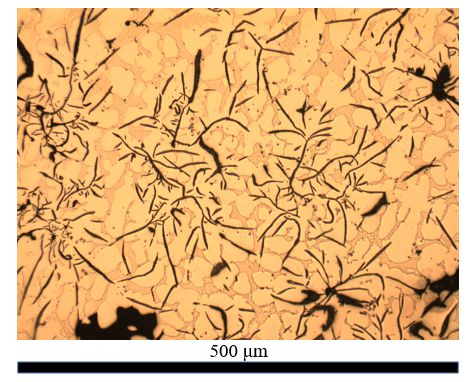
\includegraphics[scale=0.6]{10X.png}
\caption{10x before etching}
\end{subfigure}
\begin{subfigure}{0.335\textwidth}
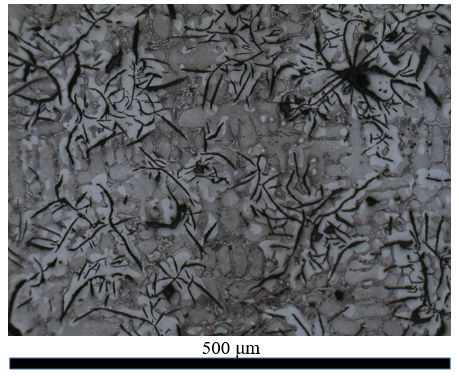
\includegraphics[scale=0.6]{10X_01.png}
\caption{10x after etching}
\label{10_after_etching}
\end{subfigure}
\begin{subfigure}{0.335\textwidth}
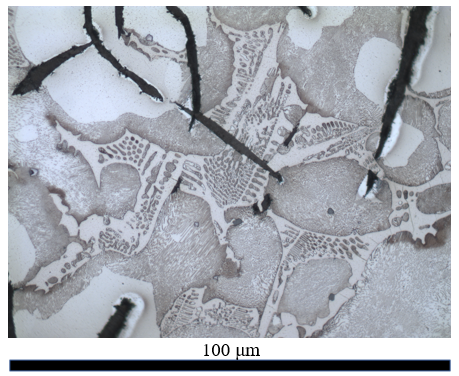
\includegraphics[scale=0.6]{50X_05.png}
\caption{50x after etching}
\label{50_after_etching}
\end{subfigure}
\caption{Optical Microscopy of grey cast iron polished surface.}
\label{optical_side}
\end{figure}
\subsection{Microscopy characterisation of fractured surface of grey cast iron}
After fracturing the specimens, the characterisation of the fractured surface is performed using an optical and a scanning electron microscope (SEM). It will allow for the identification and analysis of the porosity and graphite content at the fractured surface. Figure \ref{optical_fractured} and \ref{SEM} display the optical and SEM microscopy images of a specimen that underwent cyclic fatigue loading at 100 MPa. The optical images are used for an estimation of a range of pore sizes that are present on the fractured surface. The SEM images are captured at three different magnifications, utilizing back-scatter electrons to reveal the Z contrast and chemical composition. Graphite appears black in these images, and beach marks, which are indicative of cyclic fatigue fracture surfaces, were searched for after. The analysis of the images can be seen in section \ref{Image_analysis}.

\begin{figure} [ht]
\begin{subfigure}{0.335\textwidth}
\includegraphics[scale=0.27]{2 kn Top.png}
\caption{Top}
\end{subfigure}
\begin{subfigure}{0.335\textwidth}
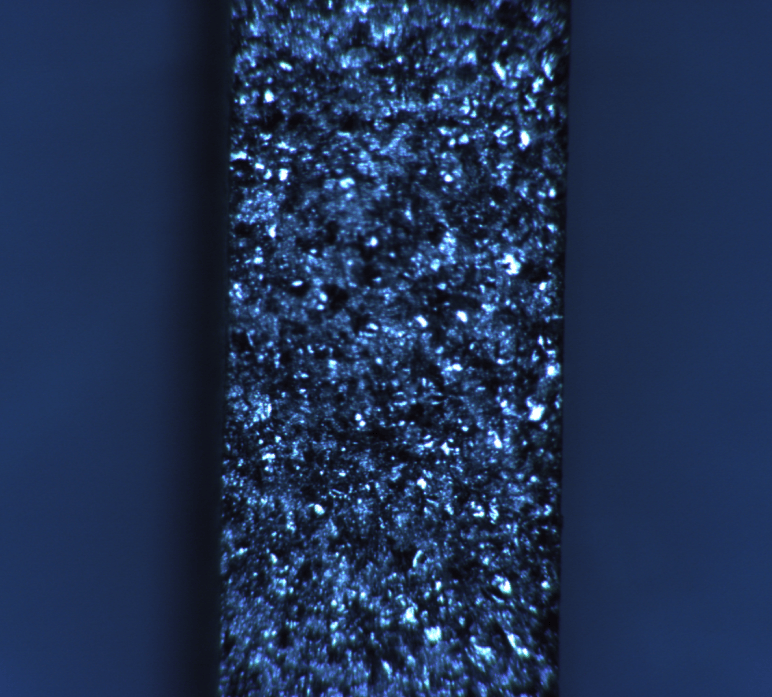
\includegraphics[scale=0.27]{2 kN Middle.png}
\caption{Middle}
\end{subfigure}
\begin{subfigure}{0.335\textwidth}
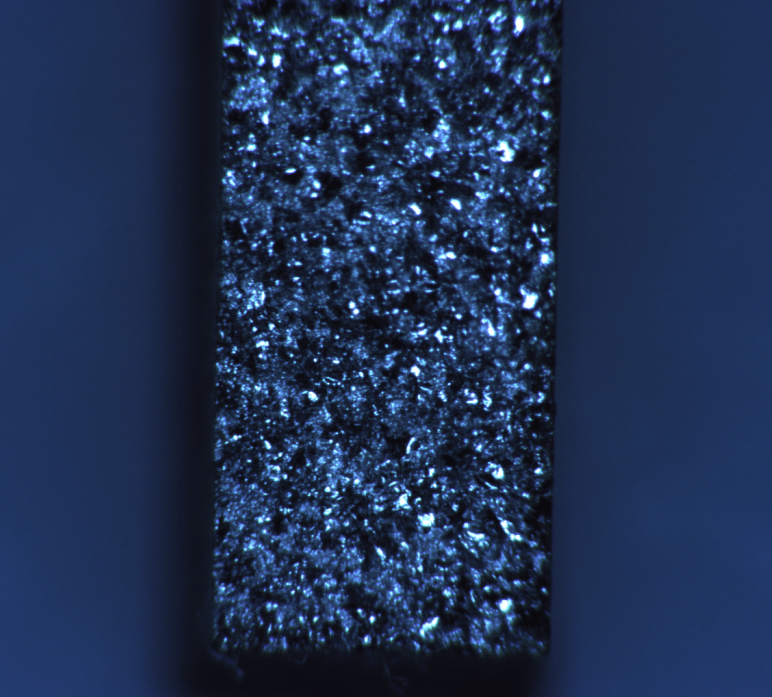
\includegraphics[scale=0.27]{2 kN Bottom.png}
\caption{Bottom}
\end{subfigure}
\caption{Optical Microscopy of fractured surface of specimen undergone cyclic loading at 100 MPa split into three parts.}
% 2 kN sample
\label{optical_fractured}
\end{figure}
\begin{figure} [ht]
\begin{subfigure}{0.335\textwidth}
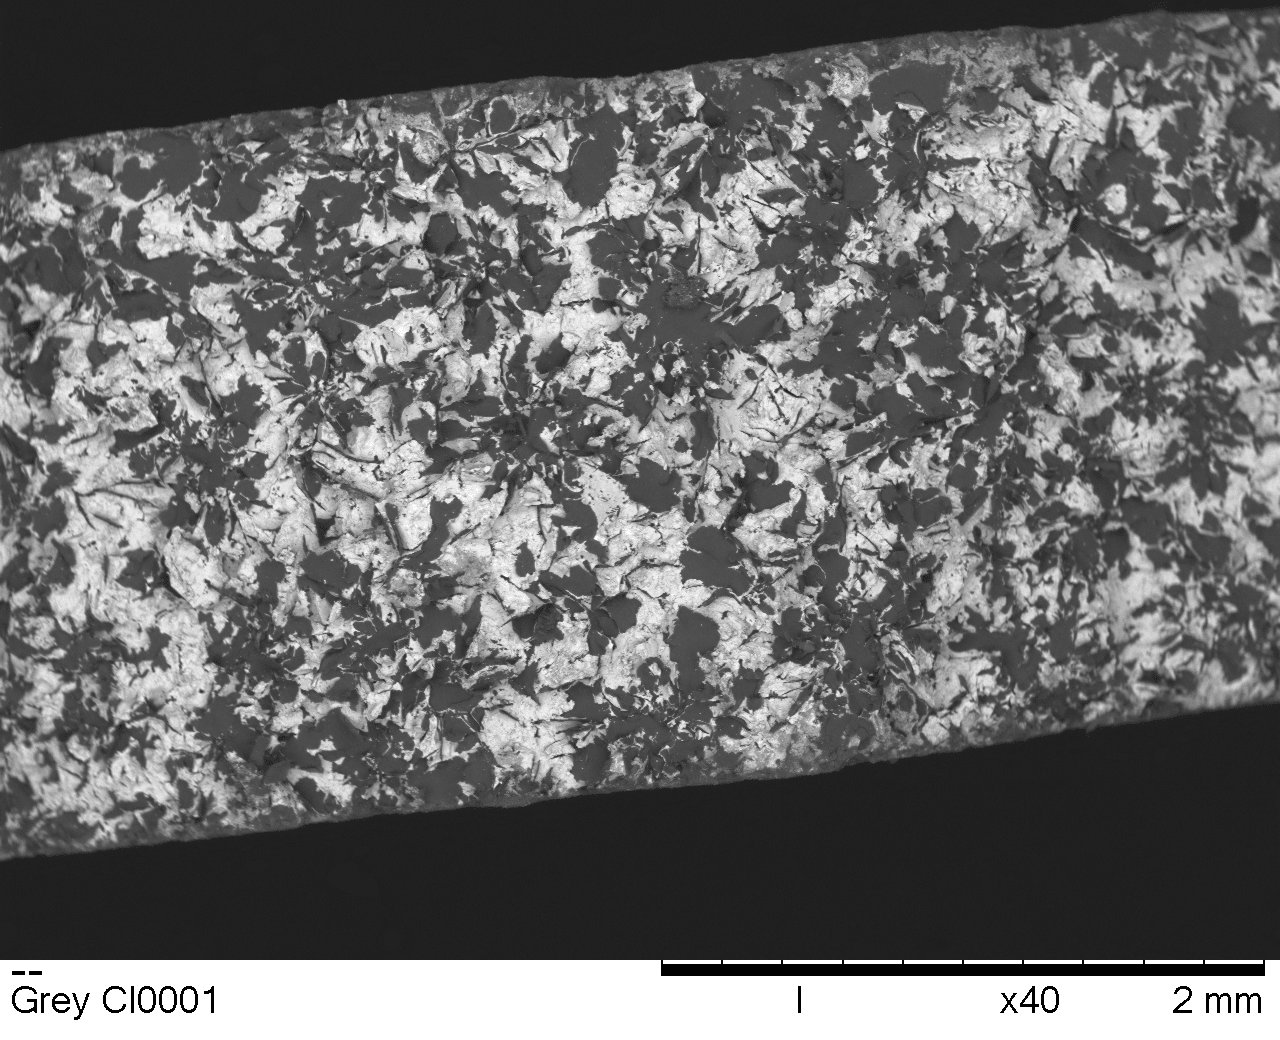
\includegraphics[scale=0.32]{Grey CI0001(x40).png}
\caption{x40}
\end{subfigure}
\begin{subfigure}{0.335\textwidth}
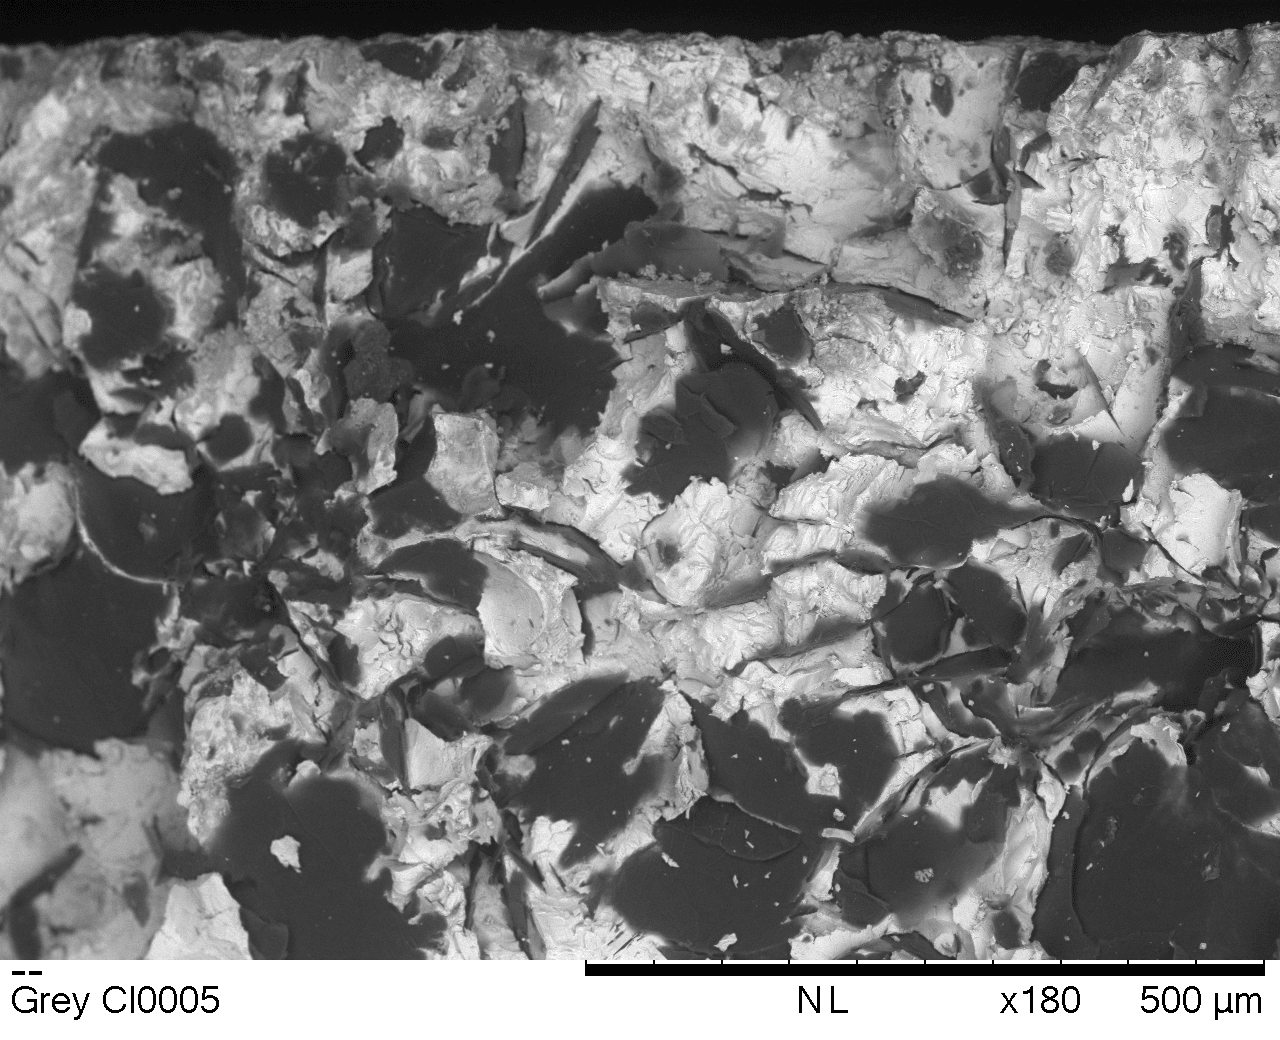
\includegraphics[scale=0.32]{Grey_CI0005(x180)(2).png}
\caption{x800}
\end{subfigure}
\begin{subfigure}{0.335\textwidth}
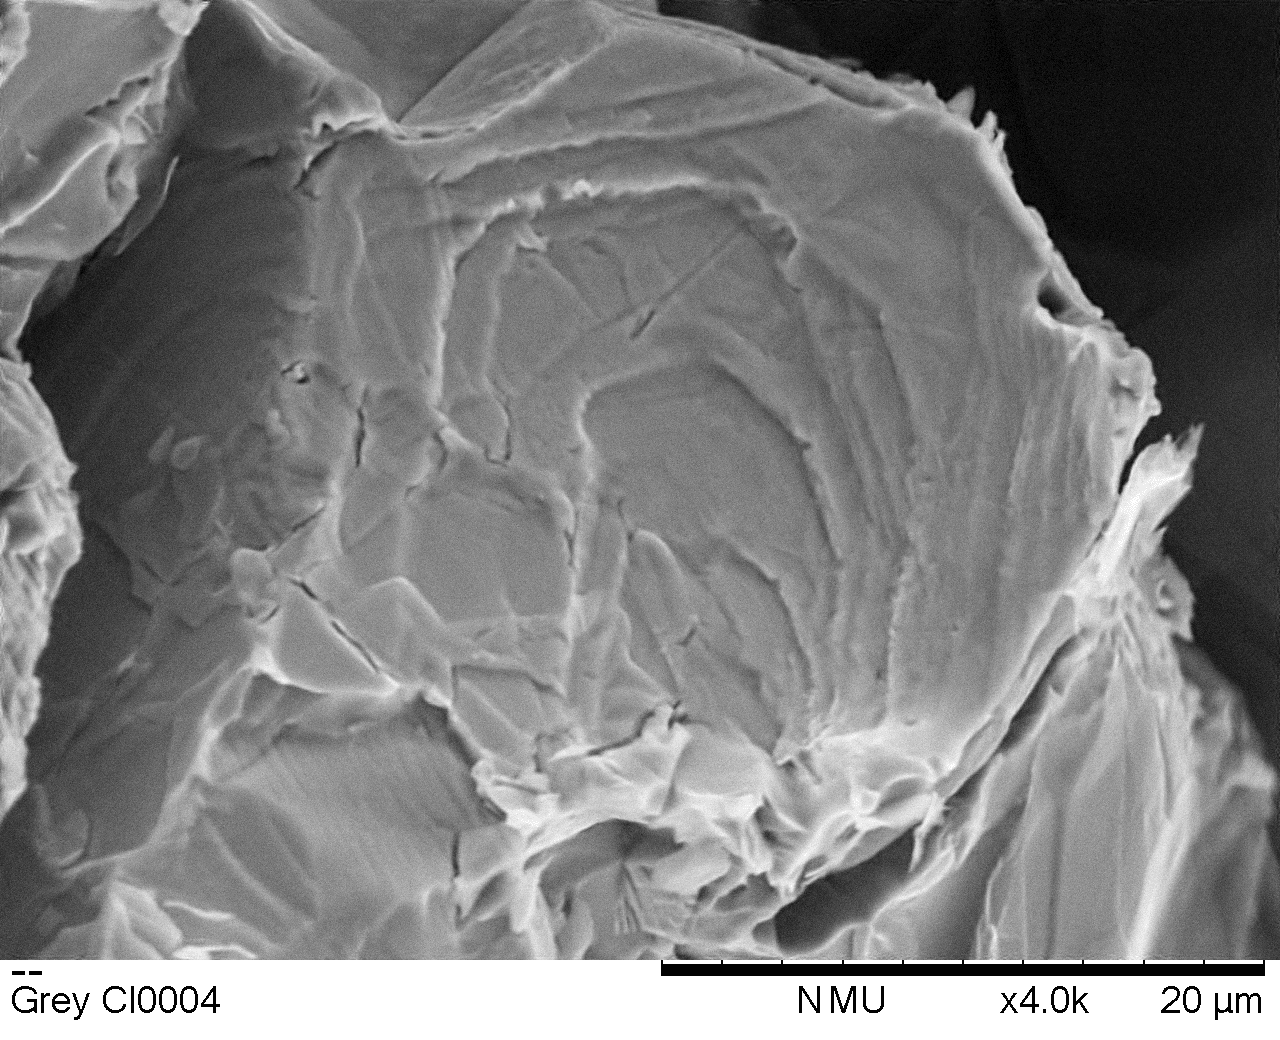
\includegraphics[scale=0.32]{Grey CI0004(x4.0k).png}
\caption{x2000}
\label{brittle}
\end{subfigure}
\caption{Scanning Electron Microscopy of fractured surface of specimen undergone cyclic loading at 100 MPa.}
% 2 kN sample 
\label{SEM}
\end{figure}

\section{Finite Element Modelling}
\subsection{Phase Field Fracture for brittle materials}
The crack geometry and fracture mechanics modelling and simulation are difficult to perform with a traditional finite element analysis method, especially in 3D. There is a need for a model that can reproduce fracture on an arbitrary mesh as it will be used to model microstructure defects. The finite element solver Abaqus employs a cohesive zone modelling method which models the crack propagation by using a traction-separation law. However, this method has limitations in capturing the complex material behavior, such as crack branching and coalescence, and the presence of pores.

\noindent Therefore, phase field models are adopted, which are mathematical models that solve interfacial problems. The fracture phase field method includes the substitution of interfaces by a partial differential equation (PDE) for an auxiliary field, the fracture phase field \cite{CARRARA2020112731}. It replaces the sharp crack surface with a diffusive zone, gradually degrading the material from intact to fully broken using the so-called crack phase field, $d$, which is a continuum variable. The crack phase field describes the sharp crack topology and takes values between 0 (undamaged material) and 1 (cracked material) as shown in figure \ref{sharp}. This is very useful because there is no need to define any interfaces in the mesh, making it possible to model the crack nucleation and propagation \cite{ambati2015review} \cite{WU20201}. The diffusive crack topology shown in figure \ref{diffusive} which includes the regularization of the crack, is governed by the length scale parameter $l$, giving for $l~\rightarrow~0$, the sharp crack topology. The choice of $l$ depends on the mesh of the specimen for proper numerical integration to occur \cite{Aldakheel2022} \cite{MIEHE2015449}.

\noindent The method for modelling the phase field fracture for brittle materials includes the coupling of the mechanical stress equilibrium equation with the phase field model of quasi-brittle fracture and damage, to calculate the linear elastic stress of damaged regions \cite{WU201772}. This approach is suitable for grey cast iron because of the brittle nature evidenced during the experiment in this project.

\begin{figure} [ht]
\begin{subfigure}{0.5\textwidth}
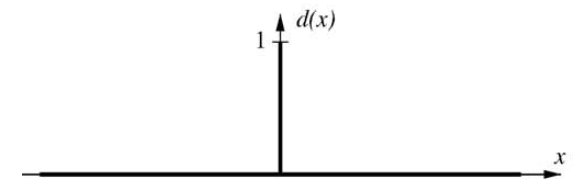
\includegraphics[scale=0.65, center]{sharp.png}
\caption{}
\label{sharp}
\end{subfigure}
\begin{subfigure}{0.4\textwidth}
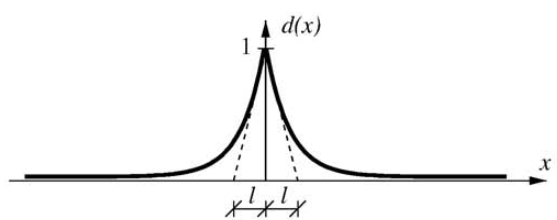
\includegraphics[scale=0.65, center]{diffusive.png}
\vspace{-7mm}
\caption{}
\label{diffusive}
\end{subfigure}
\caption{Sharp and diffusive crack topology. a) Sharp crack at x = 0. b) Diffusive crack at x = 0 modeled with the regularisation length scale $l$ in terms of the crack phase field $d$ \cite{miehe2010phase}.} 
\label{sharp_crack}
\end{figure}

\noindent Moving to the equations, the degraded elastic strain energy $\Psi(\epsilon,d)$, describes the energy related to the deformation of the material that is surrounding the crack. It entails the monotonically degradation function $g(d)$ $\in[0,1]$, which governs the material’s evolution of its mechanical behaviour. At this instance, as the phase field model evolves, it degrades the undamaged elastic strain energy $\Psi_0 (\epsilon)$, which is for instance $1/2 E \epsilon^2$ for pure tension, as it is multiplied by $g(d)$ which is equal to $(1-d)^2$. The degraded elastic strain energy density, $\Psi(\epsilon,g(d)) = g(d) \Psi^+ + \Psi^-$, is decomposed additively to separate the tensile contributions of the strain energy, $\Psi^+$, and the compressive contributions of the strain energy that act on the material, $\Psi^-$. This is done by the strain spectral decomposition that is shown in (\ref{Psi_plus_minus}). This choice allows to discriminate between the tensile load, that causes the fatigue failure, and the compressive load, which does not cause any failure. The terms $\epsilon_{1}, \epsilon_2, \epsilon_3$ represent the eigenvalues of the strain tensor.

\begin{equation}
\Psi^\pm = \lambda\left\langle \epsilon_1 + \epsilon_2 + \epsilon_3 \right\rangle_\pm^2/2 + \mu\left( \langle \epsilon_1 \rangle_\pm^2 + \langle \epsilon_2 \rangle_\pm^2 + \langle \epsilon_3 \rangle_\pm^2 \right) \ ,
\label{Psi_plus_minus}
\end{equation}
where $\lambda$ is the bulk modulus, and $\mu$ is the shear modulus of the material.
A history variable, $H$, representing the maximum energy density over the time interval $t=[0,t_0]$, where $t_0$ represents the current time step, must be defined to prevent crack healing:
\begin{equation}
H=\textrm{max}_t(\Psi^+ ) \ .
\label{History}
\end{equation}
The total free energy $F$ in (\ref{free energy}) consists of the elastic and fracture surface energy. The $g_c$ [$\textrm{J}/\textrm{m}^\textrm{2}$] parameter corresponds to the Griffith’s critical energy release rate (or fracture energy), which represents the critical value of the elastic energy at which a crack will propagate through a material. It will be calibrated by comparing with mechanical tests. The $a(d)$ term is the crack geometric function and equals to the quadratic function $d^2$.
\begin{equation}
F=g(d)H+\Psi^-+\frac{1}{c_0}(\frac{g_c}{l}a(d)+l|∇d|^2)=f(\textrm{elastic})+ f(\textrm{fracture})+\frac{g_c l}{c_0}|∇d|^2 
\label{free energy}
\end{equation}
The evolution equation which determines the phase field in the case of loading and unloading is shown in (\ref{evolution}). Note that this equation implies that strain energy embedded in $H$ acts as local fracture source \cite{miehe2010phase}.
\begin{equation}
\frac{g_c}{l}[d-l^2\Delta d] = 2(1-d)H
\label{evolution}
\end{equation}

\subsection{Extension of the model to cyclic fatigue}
The phase field model that was described beforehand is extended to account for the cyclic loading effect on the dogbone specimen. The load applied through the pull of the displacement is altered to be sinusoidal, performing 1 cycle per second. A relationship between $N_f(\sigma_{\textrm{max}}(t))$ and $\sigma_{\textrm{max}}(t)$ is extracted from the experimental results that relates the maximum alternating stress with the number of cycles to failure to be incorporated into the model. Afterwards, during the simulation, where the load is alternating between the constant maximum and minimum stress, a history variable, $\sigma_{\textrm{max}}$, is specified to track the positive maximum value of the stress. 
%as shown in figure \ref{one_element_alternating}. 
After that, Miner's rule is applied to degrade $g_c$, as described in the following. Miner's rule variable, $k$, is frequently used in engineering to predict the fatigue life of a component subjected to cyclic loading. It assumes that the total damage accumulated by a component during its lifetime is expressed as the summation of the damage caused by each individual loading cycle from 0 to $t$. The damage is the ratio of the number of cycles performed during one cycle of the simulation to the number of cycles to failure of that stress amplitude as shown in (\ref{miner}) \cite{SUN201416}. The number of cycles per second performed, $\frac{dN}{dt}$, is an input value and the number of cycles to failure, $N_f(\sigma_{\textrm{max}}(t))$ is the S-N curve data of the material analysed. $k$ is a function of time and it is given by:
\begin{equation}
k (t) = \int_{0}^{t} \frac{\frac{dN}{dt}\cdot~dt}{N_f(\sigma_{\textrm{max}}(t))} \ . 
\label{miner}
\end{equation}
This method assumes that the damage caused by each loading cycle is independent of the damage effect caused by other loading cycles.
If the Miner's rule variable, $k$, reaches the value of 1, then the specimen is going to fail. This is represented in the model by a decrease of $g_c$ towards zero when $k$ tends to 1. The tensile elastic strain energy density $\Psi^+$ obtained after the decomposition of the total energy density, is modified using a fatigue degradation function $f(d)$ in (\ref{degradation}). Indeed, this function reduces the fracture energy $g_c$ of the specimen, allowing for the cyclic loading effects to be incorporated into the simulation. The modified tensile elastic strain energy density $\Psi^+$ is shown in (\ref{Psi plus}). The history variable $H$,  used in equation (\ref{History}) is now modified according to (\ref{H_modified}):
\begin{equation}
 f(d) = 
 \begin{cases}
 10\cdot(1-k) & k > 0.9 \\
 1 & k < 0.9
 \label{degradation}
 \end{cases}
\end{equation}
\begin{equation}
\Psi^+_{\textrm{cyclic}}= \frac{\Psi^+}{f(d)}
\label{Psi plus}
\end{equation}
\begin{equation}
H = \textrm{max}_t( \Psi^+_{\textrm{cyclic}} ) \ .
\label{H_modified}
\end{equation}
Therefore, the total free energy $F$ in (\ref{free energy}) includes the modified history variable to account for the cyclic loading effects as the simulation progresses. This will be able to reproduce crack nucleation and propagation on the surface of the specimen due to cyclic loading. This shows that the extension of the phase field fracture model to the case of cyclic fatigue was performed, achieving objective \ref{O4}. 

\section{Analysis of the experimental results}

\subsection{S-N graph parameterisation}
\label{S-N analysis}
The grey cast iron experimental literature data of the fatigue testing are statically analysed for the construction of a linear equation that relates the stress, with the number of cycles to failure. The goal of this linear regression is to find a straight line that best describes the relationship between the two variables, in order to inform the $N_f(\sigma_{\textrm{max}}(t))$ function in (\ref{miner}). The two variables consist of: one that is considered the dependent variable, which is the constant maximum stress amplitude applied during the experiment, $\sigma_{\textrm{max}}(t)$, and one that is considered the independent variable, which is the number of cycles that the specimen had undergone before failing, $N_f(\sigma_{\textrm{max}}(t))$. This will ensure that the model is able to reproduce the grey cast iron experimental literature data. The linear regression performed, was able to produce a straight line, its equation, and the related confidence intervals, as shown in figure \ref{regression} and equation (\ref{sigma}). When the number of cycles to failure variable becomes the subject of the formula, it results in (\ref{number of cycles}) and allows for its prediction at different stress amplitudes. The variables $p_1$ and $p_2$ are the slope and y-intercept of the straight line respectively, with $p_1=-25.0552$ and $p_2=206.5335$ respectively.
\begin{equation}
\sigma_{\textrm{max}}(t) = p_1\cdot log_{10}(N_f(\sigma_{\textrm{max}}(t))+p_2)
\label{sigma}
\end{equation}
\begin{equation}
N_f(\sigma_{\textrm{max}}(t)) = 10^{((\sigma_{\textrm{\tiny{max}}}(t)-p_2)/(p_1))}
\label{number of cycles}
\end{equation}
\begin{figure} [ht]
\centering
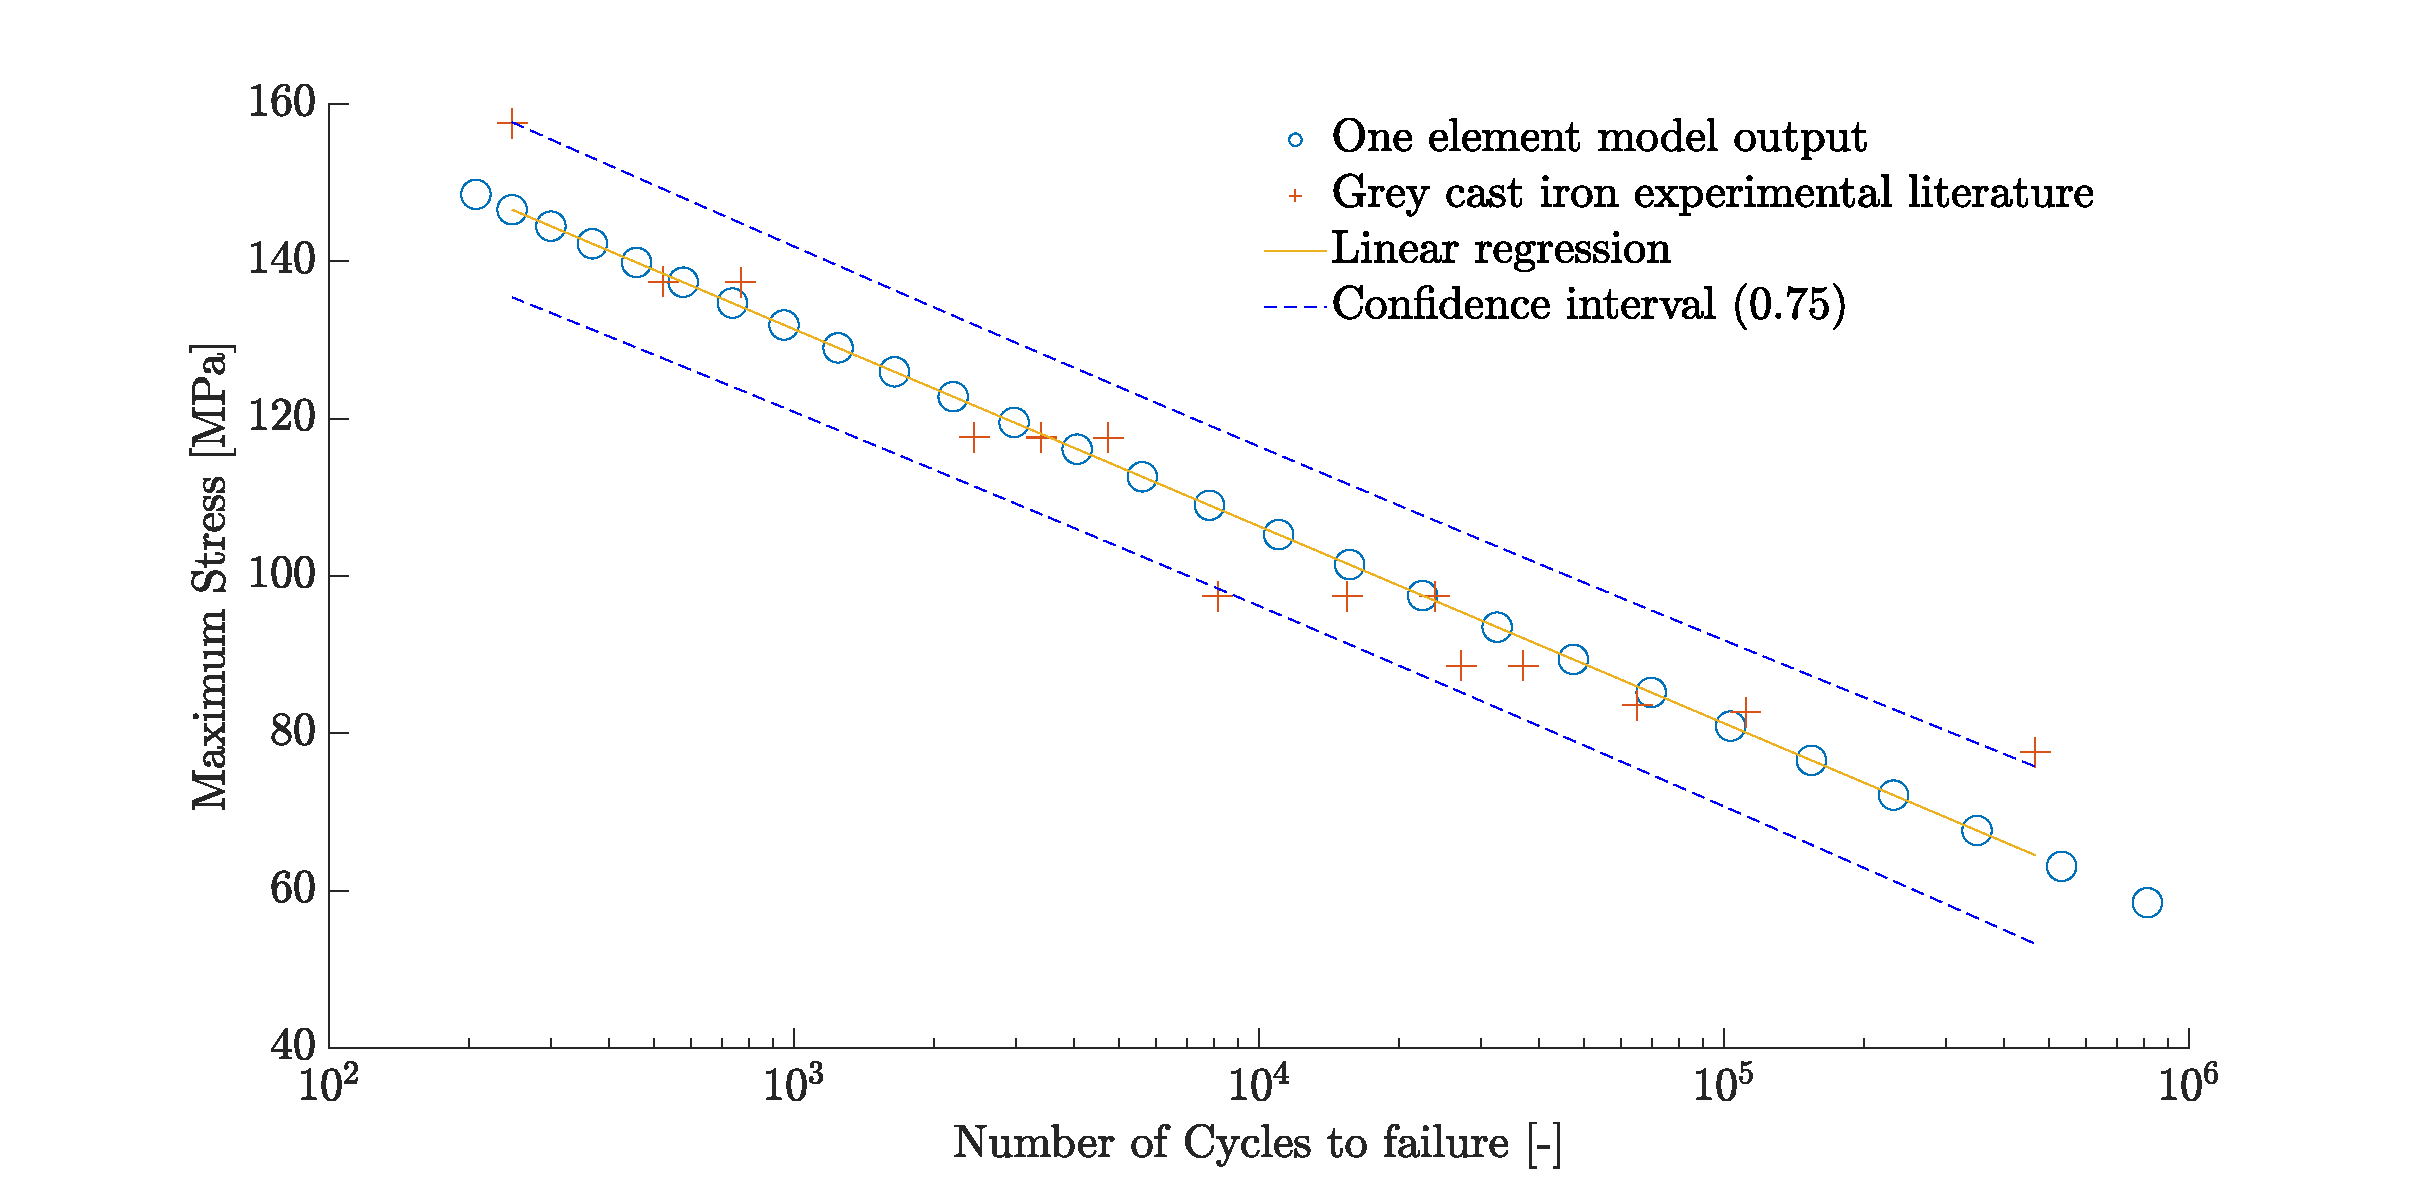
\includegraphics[width = 17cm]{Linear_regression.eps}
\caption{Linear regression and confidence intervals of the grey cast iron experimental literature data.}
\label{regression}
\end{figure}

\subsection{Image Analysis}
\label{Image_analysis}
The optical microscopy of the polished side surfaces were analysed, where graphite flakes surrounded by the pearlitic matrix was observed. This verifies that the specimen material is grey cast iron due to the high percentage of graphite and the way the flakes are distributed. Based on the ASTM A247-19 (2019) standard \cite{ASTM:A247}, graphite is classified to range from A to C, with type B being the most frequent. As most of the microstructure is pearlite, this demonstrates a moderate cooling rate. If the cooling rate had been higher, more cementite and smaller graphite flakes would have been produced. Using a MATLAB-based image-processing tool to highlight the dark colour of graphite, an average content of about 7.5\% was identified. This is consistent with the typical range of $6\%-10\%$ for grey cast iron. 

\noindent The SEM microscopy images of the fractured surface of the specimen are analysed through MATLAB to provide information on the fraction of graphite that is present in the specimen's fractured surface. After performing the analysis, a graph of the fraction of graphite against the different magnifications is shown in figure \ref{graphite fraction}, as well as an SEM image presenting how the dark colour of graphite is differentiated from the matrix. Different regions of the fractured surface were investigated. Figure \ref{brittle} confirms the brittle response of the grey cast iron specimens during the cyclic loading. The analysis estimated a graphite fraction of approximately 47\%, which is much larger than that of the polished side surface. This is because, in SEM, the Z element is the atomic number of an element, which determines its ability to scatter electrons, where low Z elements scatter electrons less efficiently than high Z elements, resulting in a darker back-scattered signal. Therefore, as grey cast iron is a low Z element, the back-scattered signal in the SEM was darker, indicating a higher fraction of graphite at the fracture surface than on the polished one. In addition, high accelerating voltages such as those above 20 kV, are known to have a stronger Z element effect and less topographic contrast, which refers to the variation in the height or depth of features on the surface. The accelerating voltage in this work range from 5-15 kV, and therefore the Z element effect is still present but is likely to be less pronounced than at higher voltages. This implies that the darker back-scattered signal observed in this work SEM images, is most likely due to the higher fraction of graphite at the fracture surface, rather than solely due to topographic contrast \cite{article}. This observation suggests that there may be large regions with an accumulation of graphite. However, it should be noted that without a secondary electron image and further analysis, it cannot be concluded that all the observed features are graphite. The above analysis shows that objective \ref{O3} is successfully achieved, where through SEM, the fractured surface of the specimen was investigated, in regards to the graphite content and possible origin of failure. 

\noindent The optical microscopy of the fractured surface of the specimen shown in figure \ref{optical_fractured} is analysed through Python, under the hypothesis that the morphology of the fracture surface is partially caused by pre-existing pores in the microstructure. This is corroborated by the fact that microscopy analysis of the sample surface, not reported here for brevity, are also showing a large density of pores. This allows to estimate a characteristic value of the pore size on the fracture surface, thus representing pre-existing pores in the bulk. Different length strips from the middle picture are extracted. The 1D Fourier transform is then applied on the different length strips, leading to the power spectral density (PSD), which is the measure of the distribution of energy across different length scales in a signal, and can provide information on the characteristic length scale of a porous material. Two graphs of the PSD against the length scale, where two different row strips of the image signal for each are plotted, can be seen in figure \ref{fourier}. The peaks in the plot represent the dominant length scales and patterns present in the image, and hence can be related to the pore size. However, they can only provide an estimated value, because the length scale of the peak might indicate other features inside a bigger pore or it might be related to the graphite flakes. Moving forward, the range of pore size deduced, ranges from 0.04-0.1 mm, where peaks on the 0.04 and 0.07 mm mark can be seen. Therefore, this shows that objective \ref{O2} is completed, as a suggested range of pore size on the fractured surface was estimated. The different features deduced from the image analysis will be incorporated into the finite element model as well. This will allow to observe if the model can accurately predict the decreased fatigue life that is due to them, and therefore match the experimental data of this work.

\begin{figure} [ht]
\begin{subfigure}{0.52\textwidth}
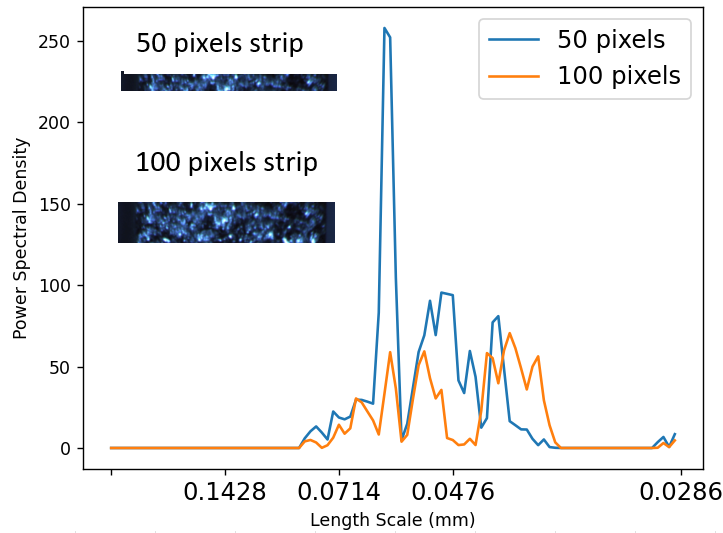
\includegraphics[scale=0.55, center]{row100.png}
\caption{50, 100 pixel size strips}
\end{subfigure}
\begin{subfigure}{0.52\textwidth}
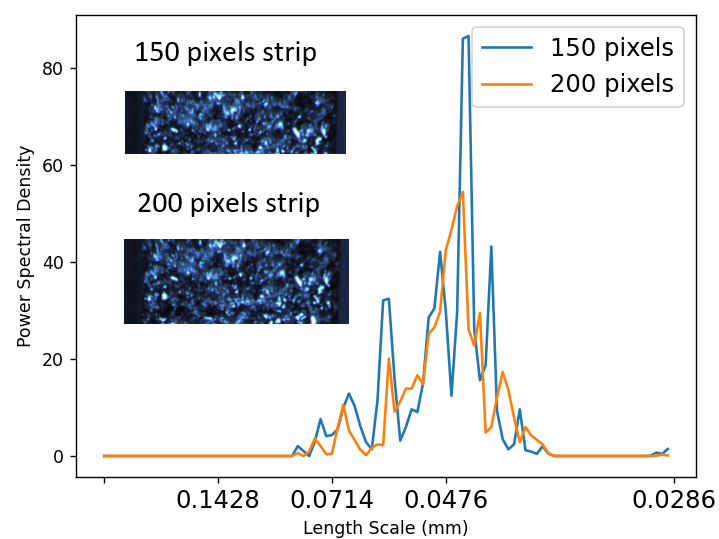
\includegraphics[scale=0.55, center]{row300.png}
\caption{150, 200 pixel size strips}
\end{subfigure}
\caption{Fourier transform of the optical microscopy image.} 
\label{fourier}
\end{figure}
\begin{figure} [ht]
\begin{subfigure}{0.52\textwidth}
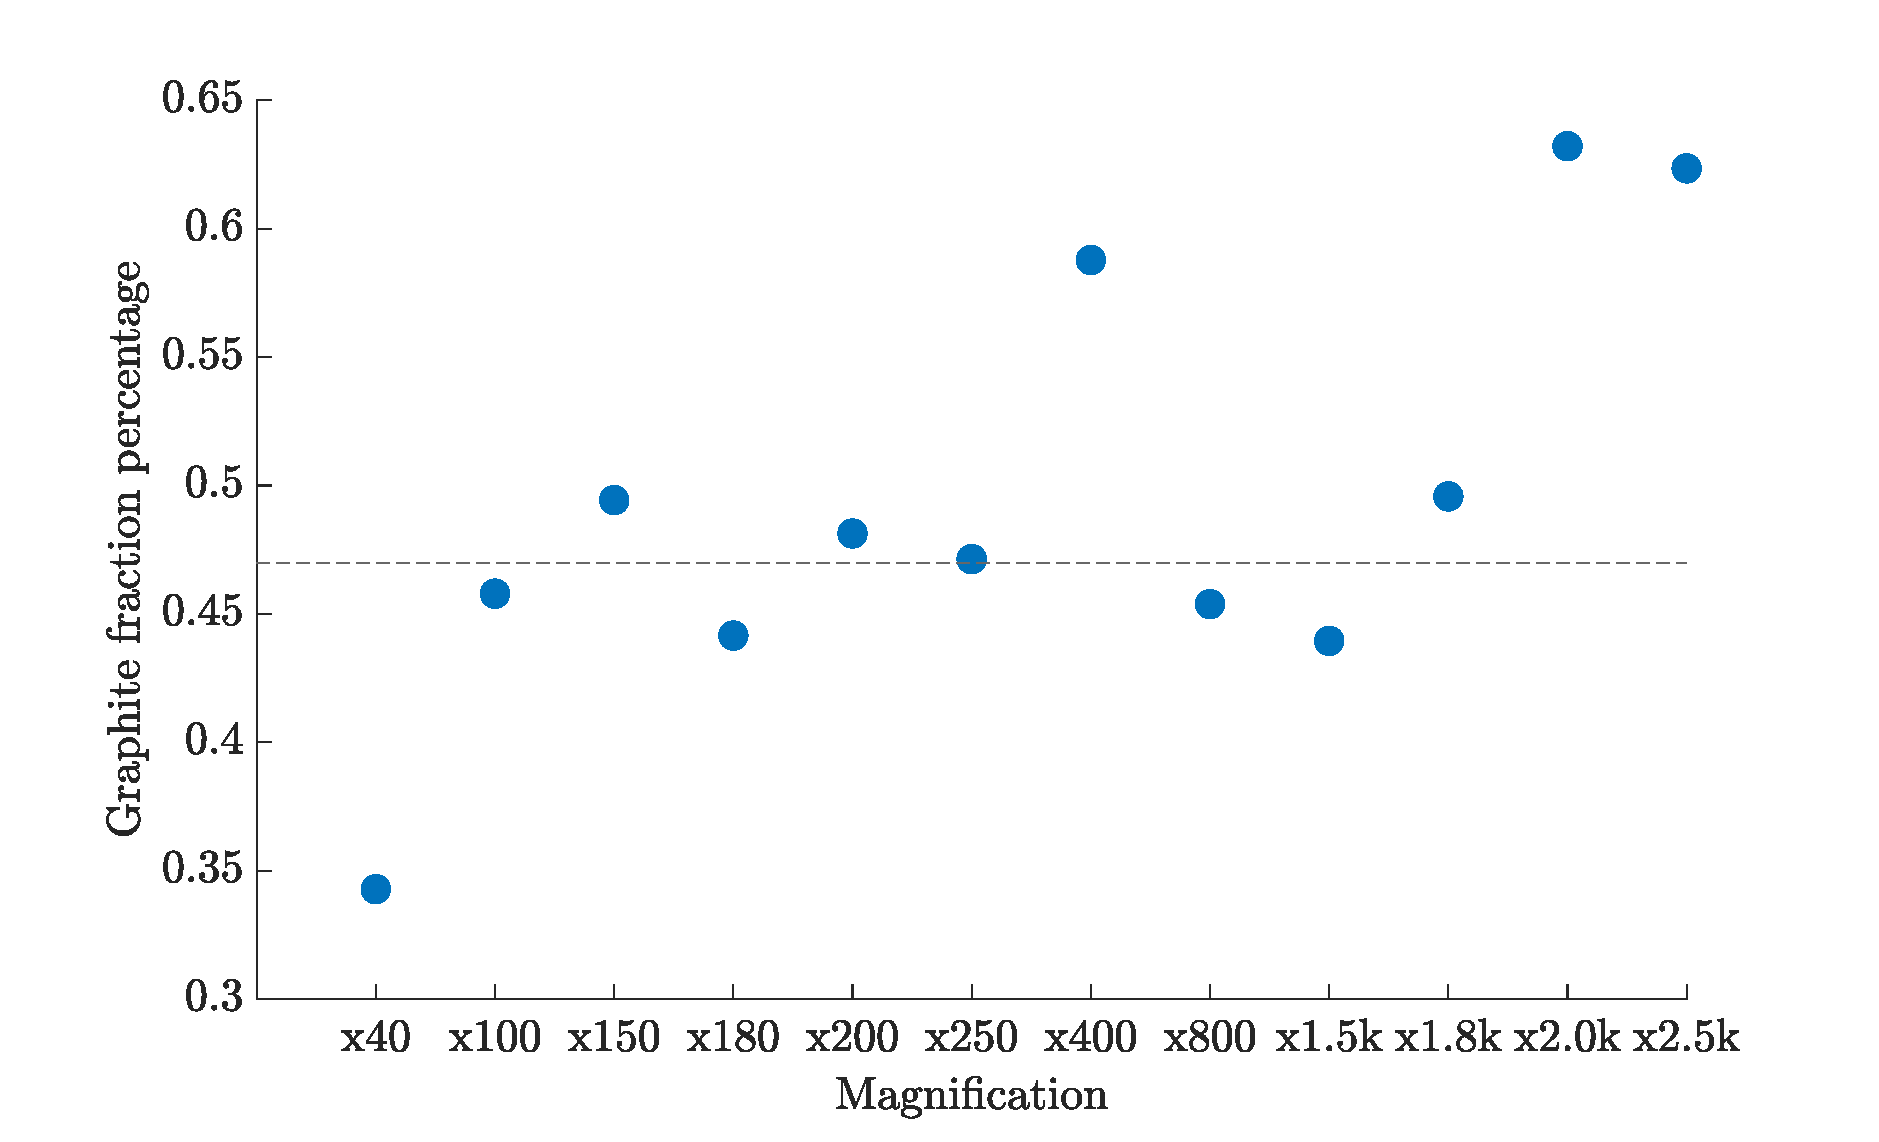
\includegraphics[scale=0.38, center]{graphite_fraction.eps}
\caption{Graphite fraction of the fractured surface}
\end{subfigure}
\begin{subfigure}{0.6\textwidth}
\vspace{6mm}
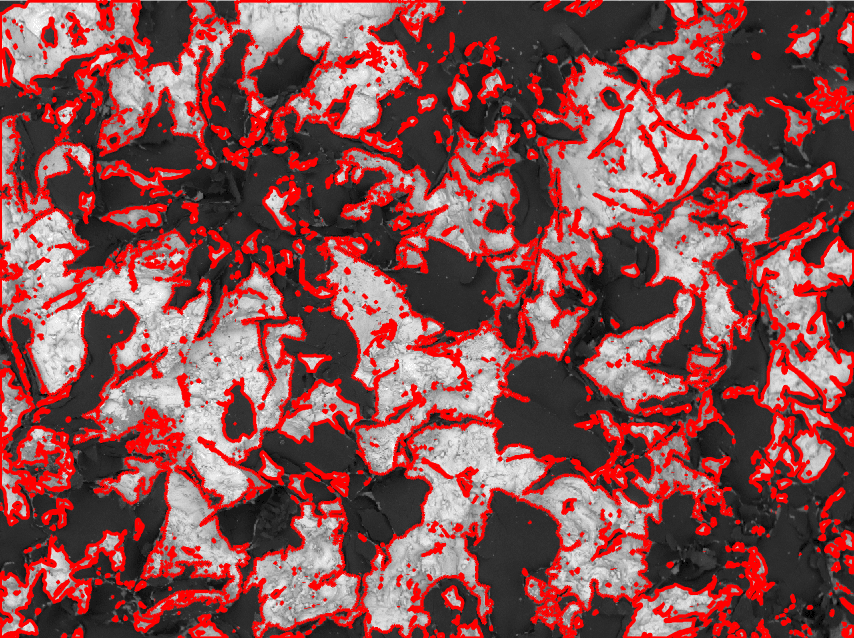
\includegraphics[scale=0.45, center]{SEM_analysis.png}
\vspace{0mm}
\caption{Differentiation of graphite dark colour with pearlite}
\end{subfigure}
\caption{Graphite fraction.}
\label{graphite fraction}
\end{figure}


\section{Simulation results}
\subsection{Model calibration}
The cyclic phase field fracture model is calibrated to be implemented on the dogbone specimen with the correct parameters. The corresponding mesh was created on Abaqus software, a three-dimensional finite element analysis tool. For more efficient simulations, a mesh of a block of $8\times 5$ mm from the center of the dogbone specimen is generated, and shown in figure \ref{ful_specimen}. Only the center part from the reduced cross-sectional area observed from figure \ref{ful_specimen} is chosen, as it is the location where the damage localises and the stress concentrates, and thus fracturing the specimen. Moreover, the specimen is allowed to contract and expand by applying a zero displacement boundary condition, perpendicular to the surface, on only three out of the five available sides, with the sixth side being the one that the load is applied on, as shown in figure \ref{center_only_mesh}. This simulates exactly how the load is applied on the center of the specimen during the actual experiment, and it is done to avoid the stress concentration at the boundary. This occurs when the regions at the fixed sides experience the highest stress concentration and hence, fracture very early, something that not happens during the actual experiment. 

\noindent In addition, two generic material constants are calibrated: the Griffith’s critical energy release rate (or fracture energy) $g_c$ $\left [\textrm{J}/\textrm{m}^\textrm{2} \right ]$, and the regularization length $l$ $\left [\textrm{m} \right ]$. The calibrated parameter is actually the ratio between the two constants, $\frac{g_c}{l}$ $\left [\textrm{J}/\textrm{m}^3 \right ]$, which represents the energy per unit volume required to initiate a crack. This ratio determines how quickly the crack nucleates, while the parameter $g_c$ determines how the crack propagates through the material. The width of this diffuse zone is proportional to the regularization length $l$, which is a characteristic length scale introduced in the model, to smooth out the sharp crack surfaces. By adjusting the value of $\frac{g_c}{l}$, the phase field model can be used to accurately predict the crack behavior in a given material \cite{miehe2010phase} \cite{kristensen2016assessment}. The regularization length $l$ is assumed to be two times bigger than the element size used for the mesh in order to interpolate the diffuse crack phase field $d$, shown in figure \ref{sharp_crack}. The fracture energy is then calibrated by ensuring that the maximum tensile stress during the first cycle, is equal to the compressive stress, where a 10\% drop is acceptable. Also, the tensile stress should drop close to zero when the specimen fractures, and the crack phase field $d$ should be able to evolve up to 1. The analysis performed to deduce the best ratio for the model created a compromise. If a large value of the ratio $\frac{g_c}{l}$ is used, it produces equal tensile and compressive stresses during the first cycle, but it does not allow for the crack phase field $d$ to evolve up to 1, giving a maximum of approximately 0.9. On the other hand, when a small value is used for the ratio, it allows for $d$ to evolve up to 1, but the tensile stress during the first cycle is reduced to more than 10\% in relation to the compressive one, which is against experimental observation. This resulted in choosing a ratio value of $10^7$ $\textrm{J}/\textrm{m}^3$ that produces approximately a 1-2\% difference between the tensile and compressive first cycle stress, and allows the crack phase field, $d$ to reach 1. Lastly, the Young's Modulus $\left [ \textrm{GPa} \right ]$ is calibrated as well, to a value of 61.04 GPa, through a linear regression. After that, the model is verified on a one element mesh and then applied on the model specimen.

\begin{figure} [ht]
\begin{subfigure}{0.5\textwidth}
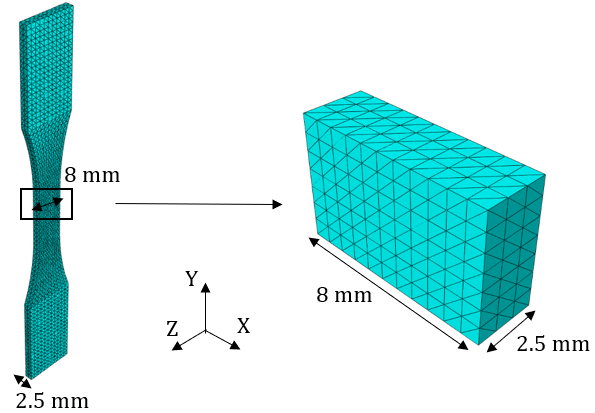
\includegraphics[scale=0.65, center]{specimen.png}
\caption{Mesh}
% /GreyCastIron/Dogbone/dogbone.i
\label{ful_specimen}
\end{subfigure}
%\hspace{-4cm}
\begin{subfigure}{0.5\textwidth}
\vspace{-3mm}
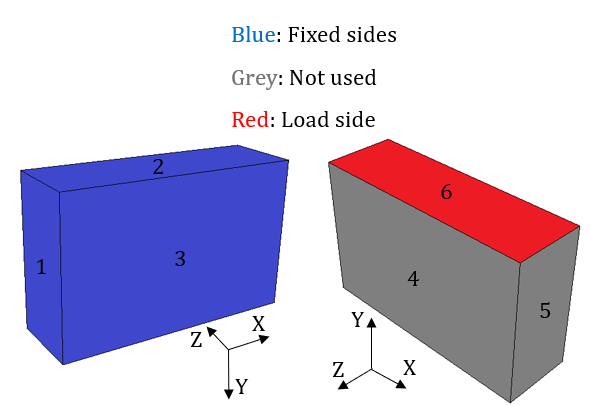
\includegraphics[scale=0.65, center]{BCs.png}
\vspace{0mm}
\caption{Boundary conditions on specimen}
\label{center_only_mesh}
\end{subfigure}
\caption{Dogbone specimen.}
\label{mesh normal}
\end{figure}

\subsection{Model verification on one element mesh}
To verify the model, a simulation with 100 MPa load amplitude is carried out. The linear regression equation (\ref{number of cycles}) is firstly verified by ensuring that the model output, specifically $\sigma_{\textrm{max}}(t)$ against the number of cycles to failure $N_f(\sigma_{\textrm{max}}(t))$, matches the regression line, as shown in figure \ref{regression}. Furthermore, when the specimen fractures, the stress must drop to a very small value close to zero, on the predicted cycle provided by the linear regression equation (\ref{number of cycles}), as shown in figure \ref{one_element_alternating}. Moreover, the Miner's rule variable, $k$, from (\ref{miner}), must indicate failure at the correct number of cycles. This suggests to confirm the number of cycles that the variable reaches 1. In addition, the fatigue degradation function $f(d)$ from (\ref{degradation}), should drop from 1 to 0 as soon as the Miner's rule variable reaches 0.9. Both variables are shown in figure \ref{miner and fatigue}. As the number of cycles per second performed, $\frac{dN}{dt}$, equals to 1000 s$^{-1}$, this implies that 1 effective cycle in the simulation, $N_e$, represents 1000 deformation cycles. Inspecting figure \ref{regression}, the model one element output data of the S-N graph is verified, as it aligns exactly on the linear regression line. Also, it can be seen that failure is suggested after approximately 17000 cycles, when a 100 MPa stress amplitude is applied. This can be clearly verified from figure \ref{one_element_alternating}, as the stress applied on the one element model, drops close to zero at 17140 cycles. In addition, from figure \ref{miner and fatigue}, the Miner's rule variable and the fatigue degradation function can be seen to reach 1 and 0 respectively at 17140 cycles. Both data suggests that the specimen failed at the correct number of cycles. The difference of the tensile and compressive stress in the first cycle is 2\%, and therefore acceptable. Moreover, the fatigue degradation function is initiated when the Miner's rule variable reaches 0.9, verifying again the model.

\begin{figure} [ht]
\begin{subfigure}{0.51\textwidth}
\centering
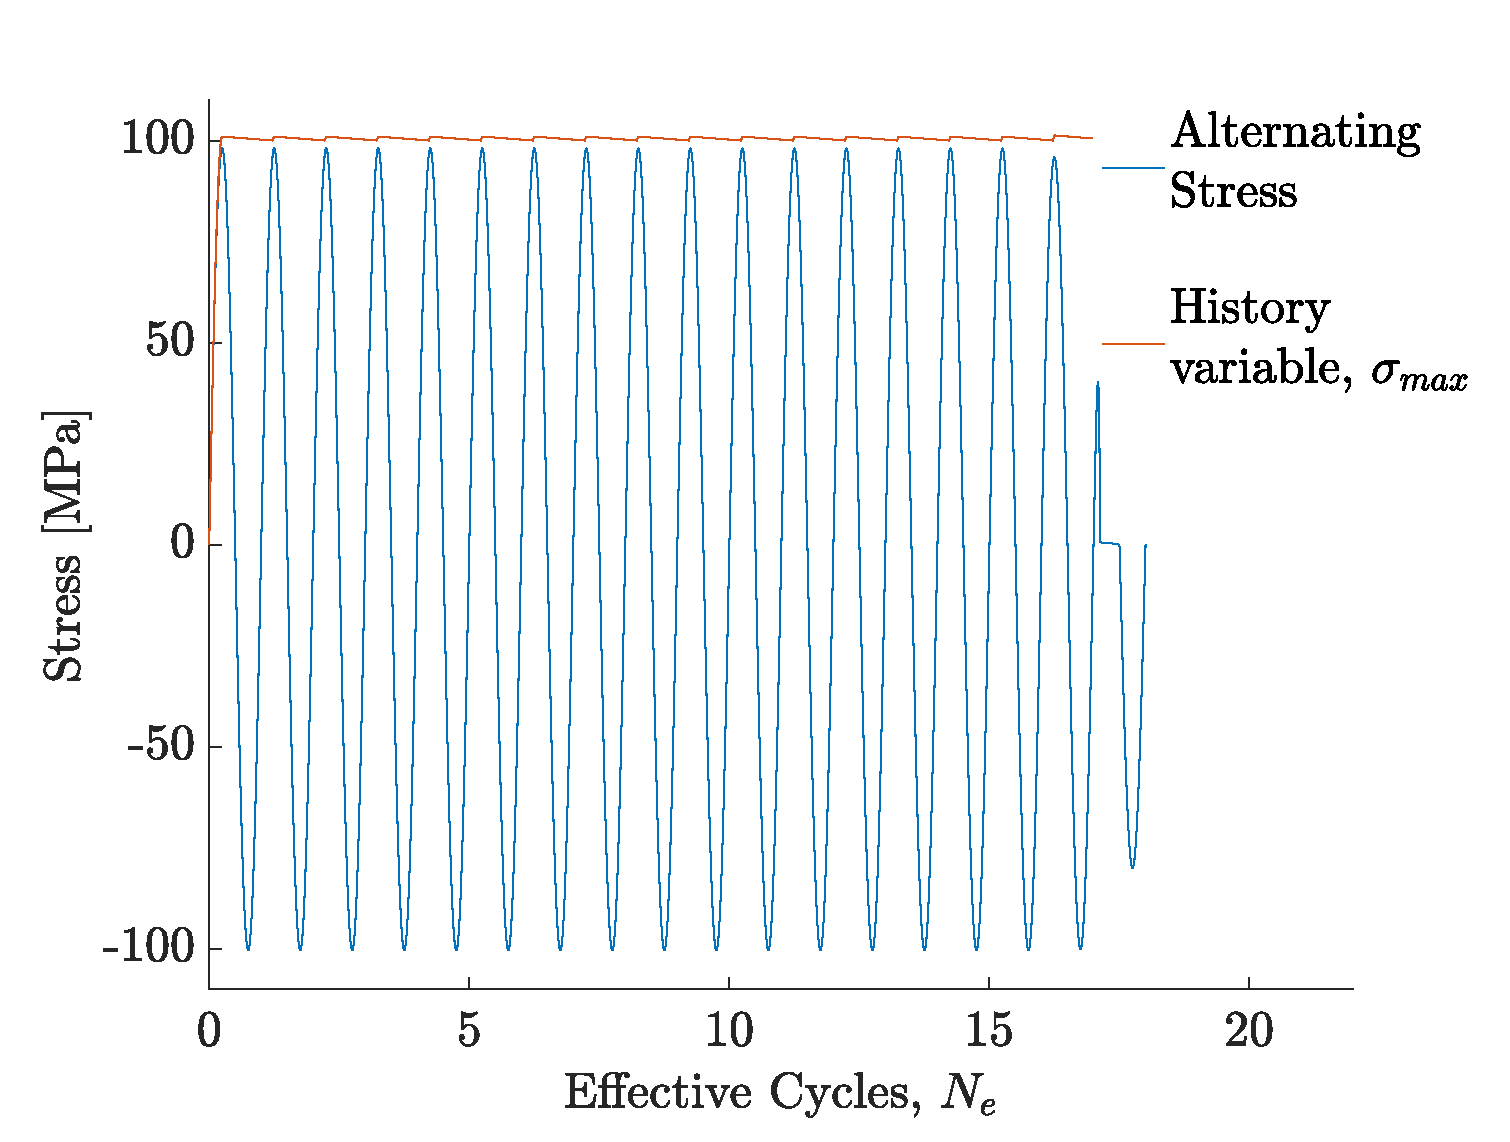
\includegraphics[scale=0.36]{stress.eps}
\caption{Alternating applied stress}
\label{one_element_alternating}
\end{subfigure}
\begin{subfigure}{0.5\textwidth}
\centering
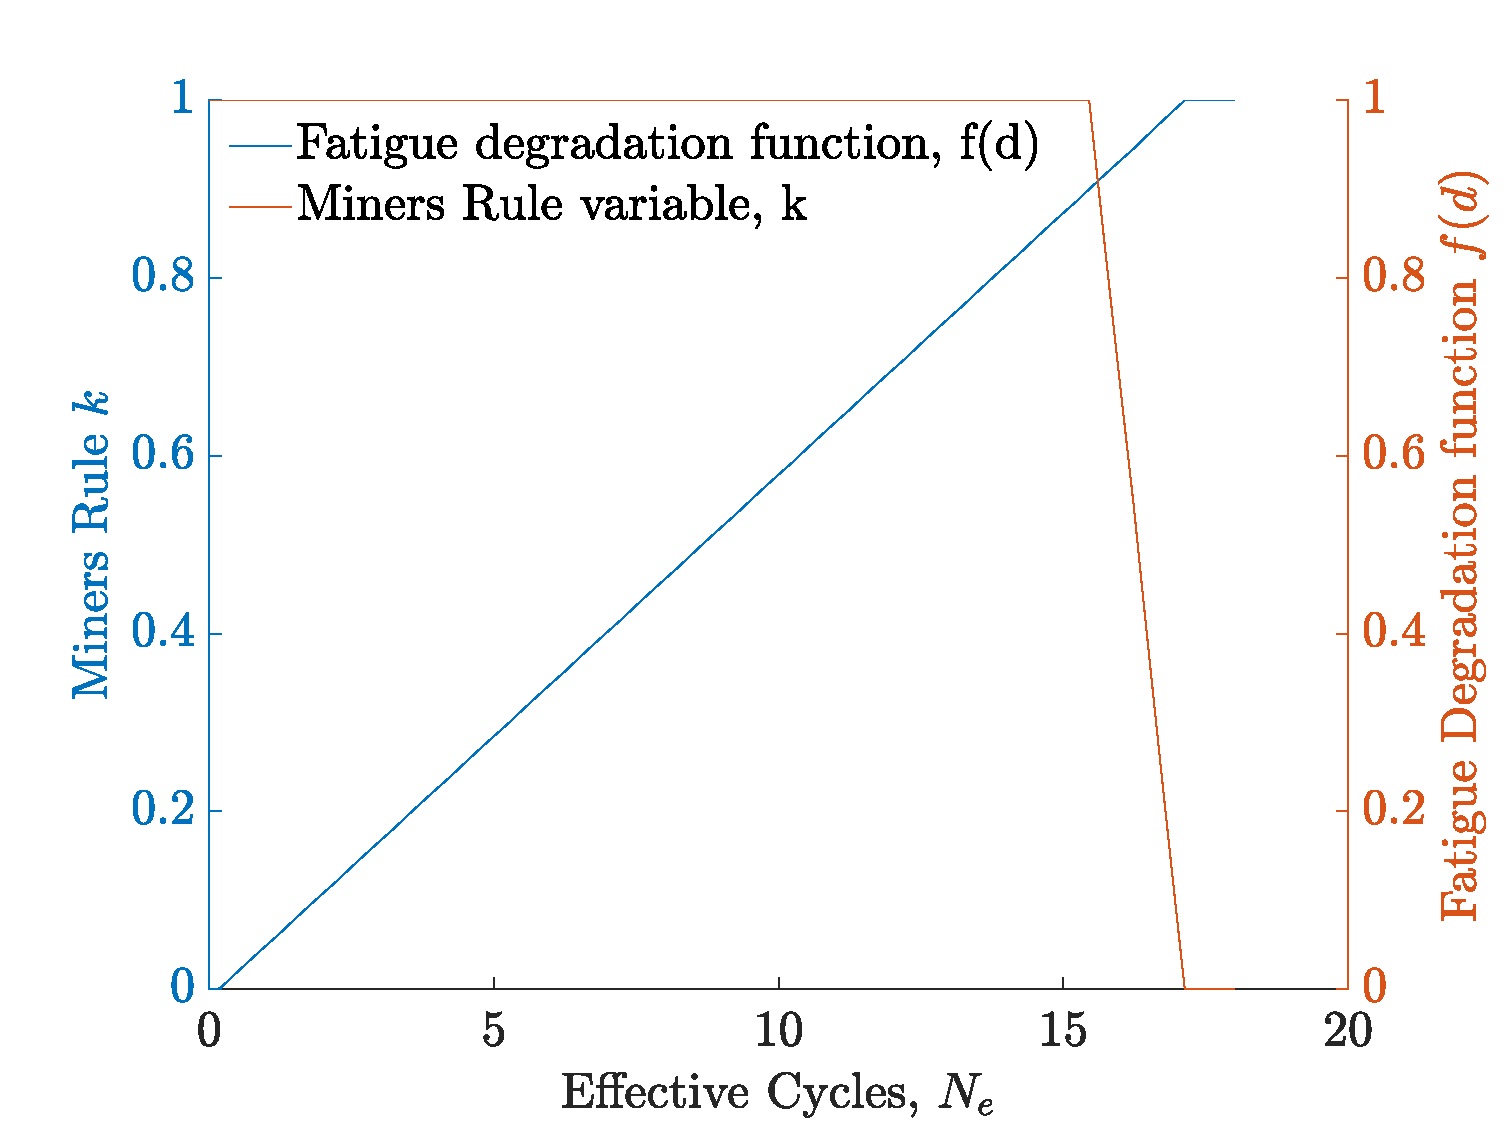
\includegraphics[scale=0.36]{miner_fatigue.eps}
\caption{Miner's rule and fatigue degradation function}
\label{miner and fatigue}
\end{subfigure}
\caption{One element model verification.}
\label{one element}
\end{figure}

\subsection{Simulation on a defect-free specimen}
The verification of the model on the one element mesh allows for its use on the specimen. A 100 MPa stress amplitude is applied. The model output line of the maximum stress,  $\sigma_{\textrm{max}}(t)$,  against the number of cycles to failure, $N_f(\sigma_{\textrm{max}}(t))$, is plotted and shown in figure \ref{model specimen S-N}. In addition, the alternating stress that is applied throughout the simulation is plotted on figure \ref{alternating stress model specimen}. From figure \ref{model specimen S-N}, it can be observed that the model output S-N graph matches the linear regression equation (\ref{number of cycles}) and shows that the specimen will fail according to the grey cast iron experimental literature data. Also, the alternating stress drops close to zero after 17200 cycles, as it can be seen from figure \ref{alternating stress model specimen}. This shows the correct cycle at which failure occurs, as estimated by the regression equation. Therefore, both data suggests that the model is working as intended on the dogbone specimen part, clearly showing that the first part of objective \ref{O6} is achieved. Consequently, it is possible now to model the micro-structural features of the grey cast iron specimen, to be able to assess their effect on the reduction of its fatigue life.

\begin{figure} [ht]
\begin{subfigure}{0.52\textwidth}
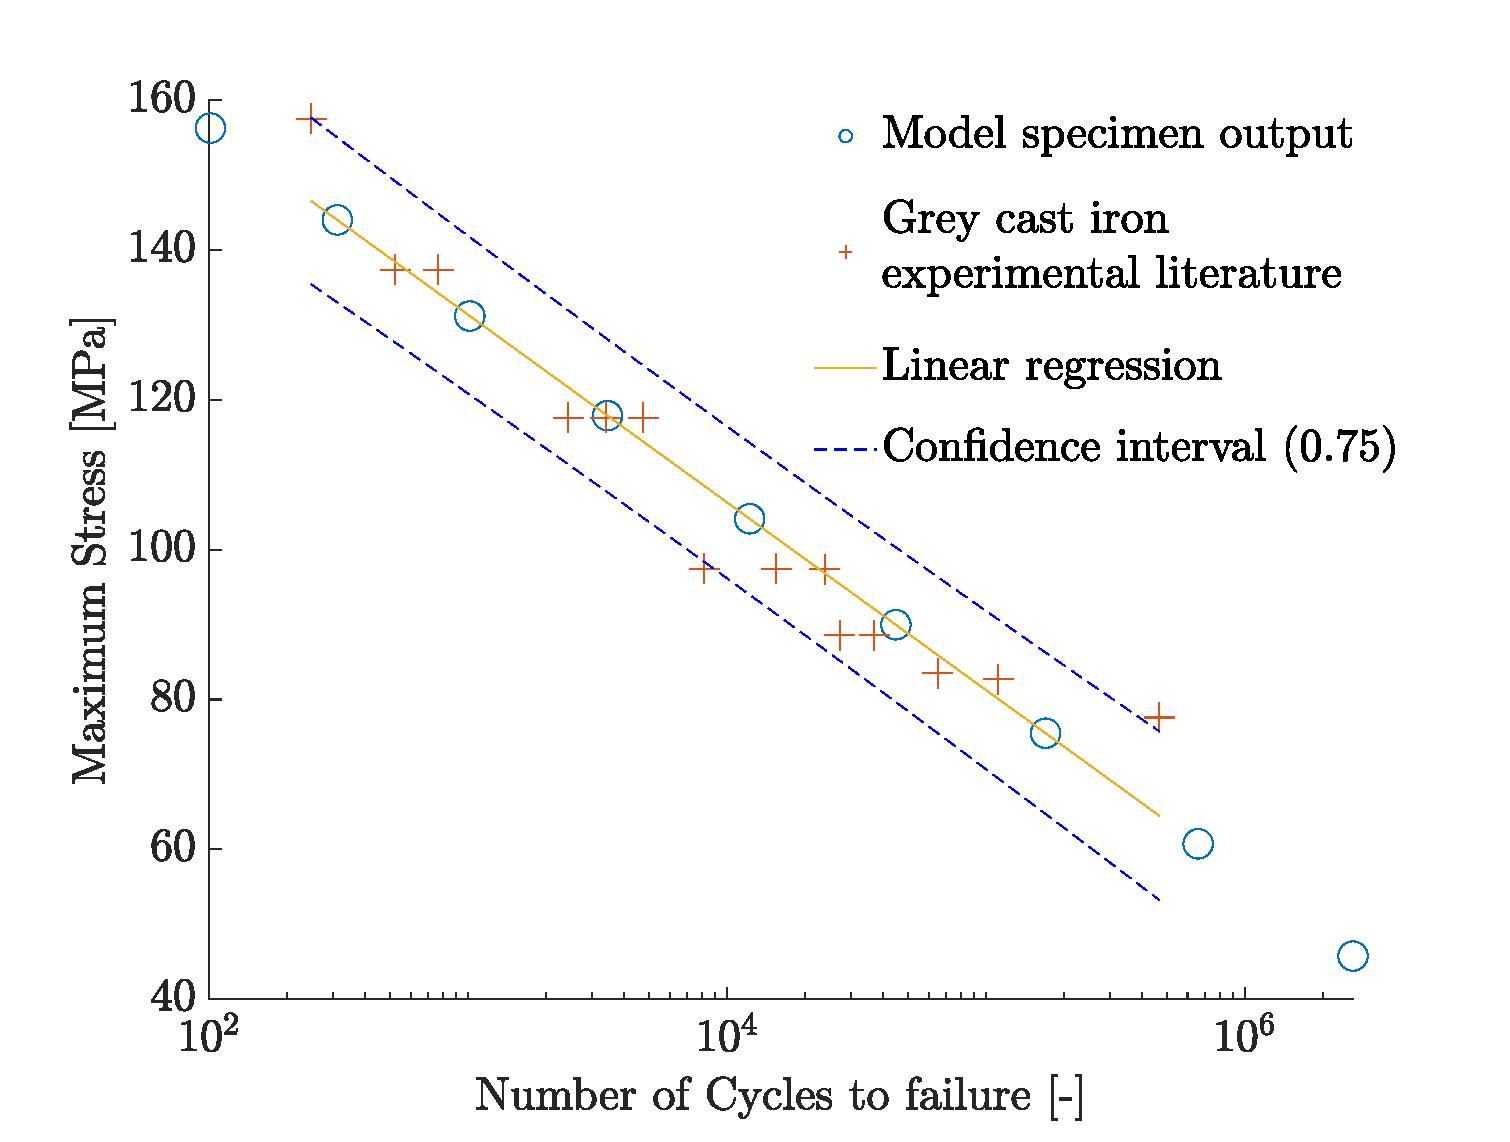
\includegraphics[scale=0.4, center]{model.eps}
\caption{Maximum stress with number of cycles to failure}
\label{model specimen S-N}
\end{subfigure}
\begin{subfigure}{0.57\textwidth}
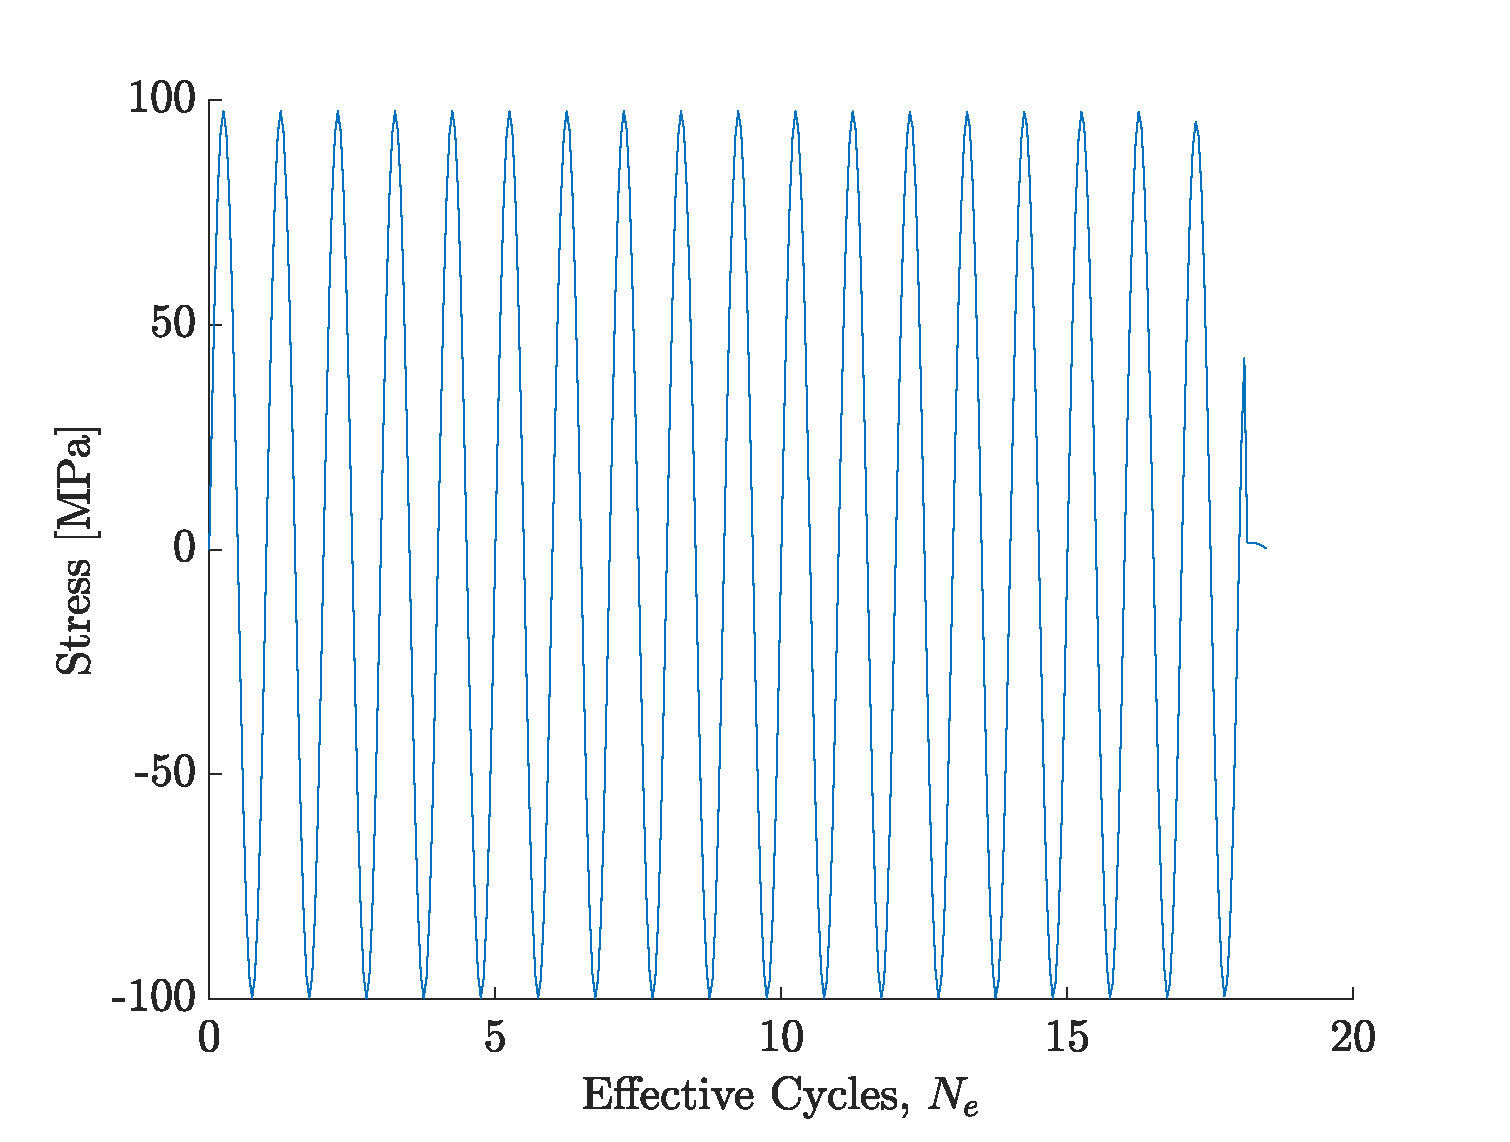
\includegraphics[scale=0.4, center]{model_stress.eps}
\caption{Alternating average stress on load surface}
\label{alternating stress model specimen}
\end{subfigure}
\caption{Defect-free model results.}
% C:\Users\Kypri\OneDrive\Documents\IRP\Simulations_nameoffile
\end{figure}

\subsection{Model with micro-structural features}
To model the effect of the features and investigate how they are affecting the fatigue life of grey cast iron, the same mesh from the block extracted from the dogbone specimen center is used. Also, a 100 MPa stress amplitude is applied, and when the average stress on the load surface decreases to 50\% of the maximum value, failure is assumed.

\noindent The optical microscopy images of the 100 MPa specimen that were analysed in section \ref{Image_analysis}, revealed a range of pore size of 0.1-0.04 mm. Therefore, different models with different pore sizes are modelled, ranging from 0.01 mm to 0.25 mm. This was done to observe if the reduction of the fatigue life of the specimen due to the different pore sizes, matches the experimental data of this work. The pore was assumed to be a circular like random shape with a known diameter located near the surface, to make it as realistic as possible. The mesh of the block specimen with a 0.1 mm pore is shown in figure \ref{pore specimen}. The number of cycles per second performed, $\frac{dN}{dt}$, equals to 100 s$^{-1}$, and therefore this implies that 1 effective cycle in the simulation, $N_e$, represents 100 deformation cycles. The alternating applied stress during the simulation is shown in figure \ref{pore alternating}. Also, the crack phase field $d$, can be observed from figure \ref{damage field} at three different number of effective cycles, $N_e$.

\noindent Moreover, the SEM microscopy images of the 100 MPa specimen, in section \ref{Image_analysis}, revealed an accumulation of graphite on the fractured surface. Therefore, to compare the effect of the pore with the effect of the graphite flake, a model specimen with a graphite flake is created. The graphite flakes were modelled to have the same size as the pores to allow for a fair comparison between them, with a range of 0.1-0.25 mm. The mesh of the specimen with the graphite flake of length 0.1 mm is shown in figure \ref{mesh graphite}. The number of cycles per second performed, $\frac{dN}{dt}$, equals to 1000 s$^{-1}$, and therefore this implies that 1 effective cycle in the simulation, $N_e$, represents 1000 deformation cycles. The elastic constant used for the graphite was equal to 40 GPa. The alternating stress of the simulation is shown in figure \ref{graphite alternating}.

\noindent Furthermore, the respective reduction of the fatigue life against the different pore and graphite flake sizes, were plotted and shown in figure \ref{reduction}.

\begin{figure} [ht]
\begin{subfigure}{0.5\textwidth}
\hspace{-8mm}
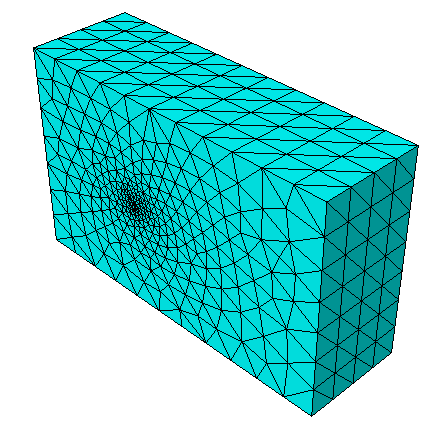
\includegraphics[scale=0.52, center]{01mm_mesh.png}
\vspace{20mm}
\caption{Mesh of the specimen with the pore}
\label{pore specimen}
\end{subfigure}
\begin{subfigure}{0.5\textwidth}
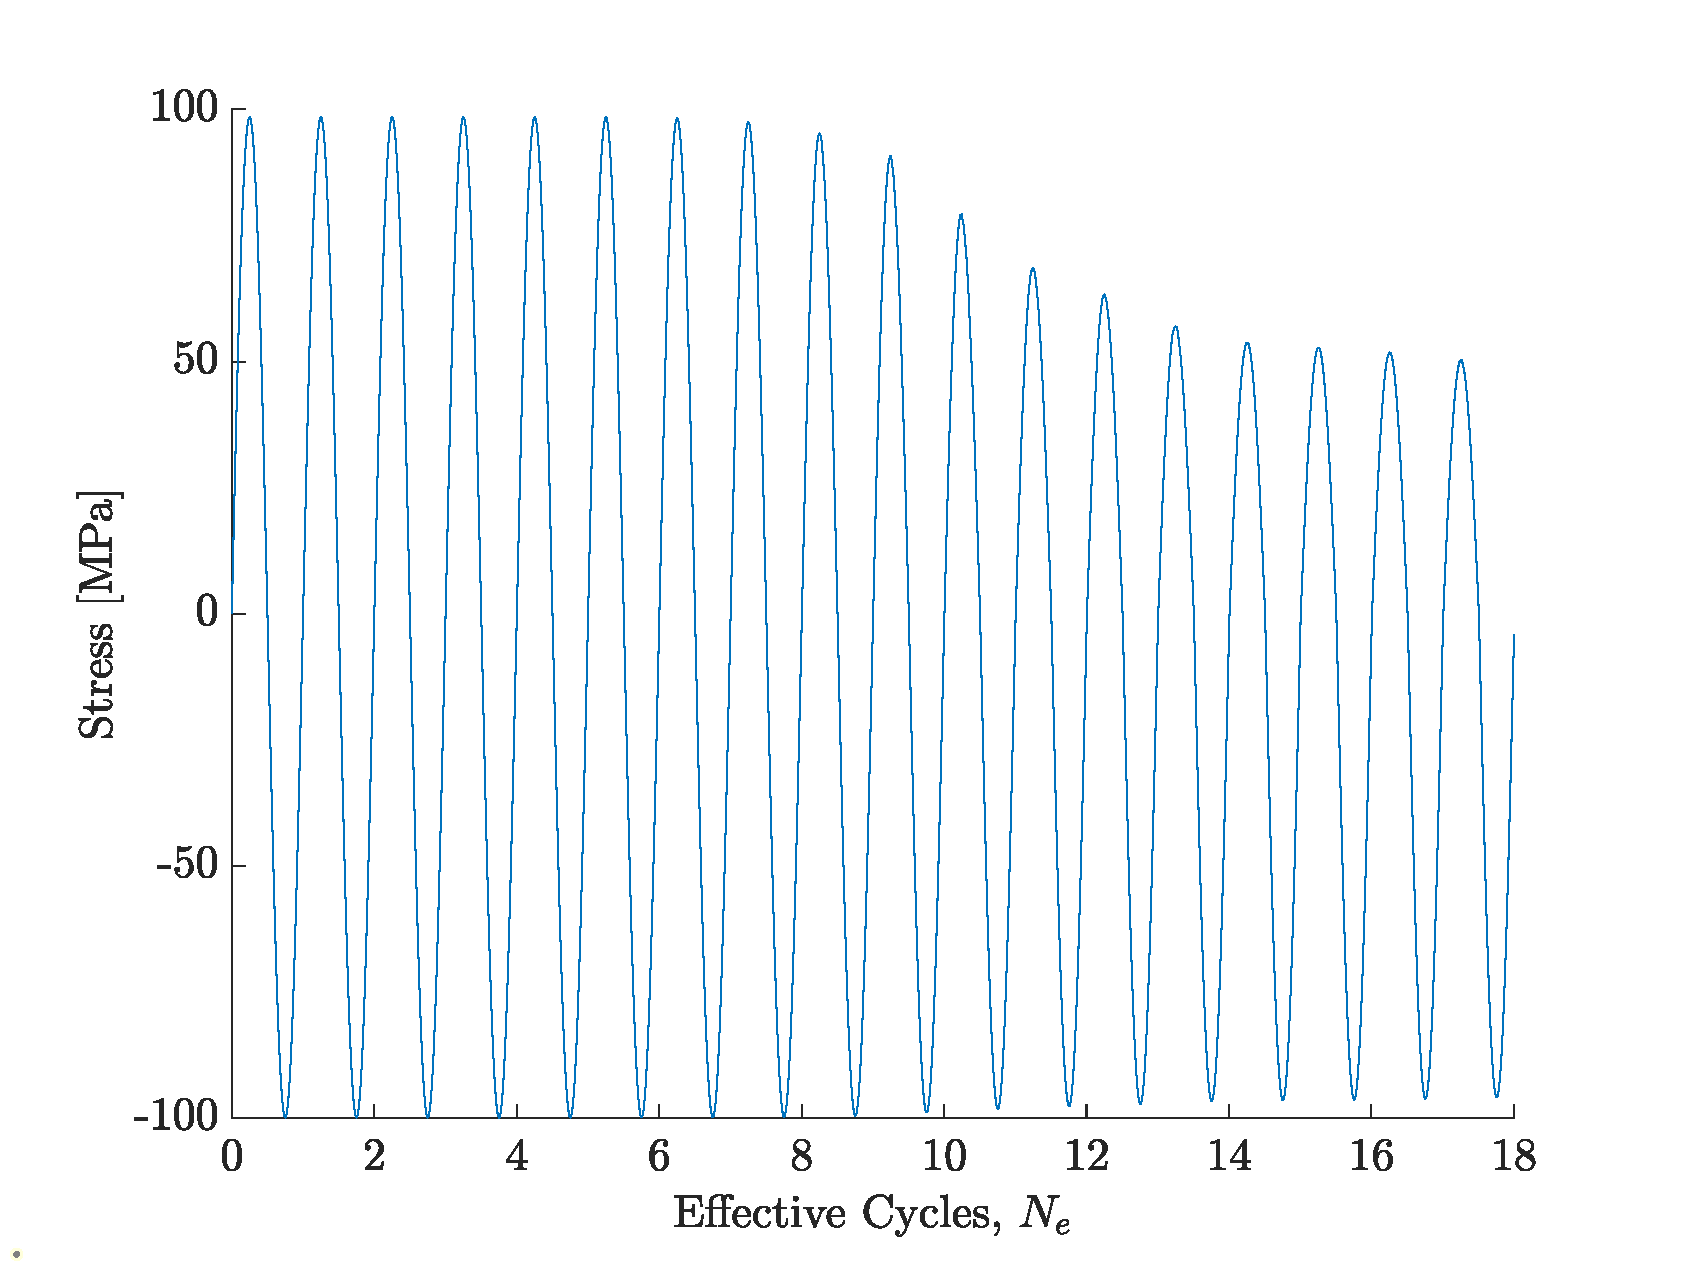
\includegraphics[scale=0.37, center]{stress_porosity.eps}
\caption{Alternating average stress on the load surface}
\label{pore alternating}
\end{subfigure}
\caption{Model with porosity.}
\end{figure}
\begin{figure} [ht]
\begin{subfigure}{0.335\textwidth}
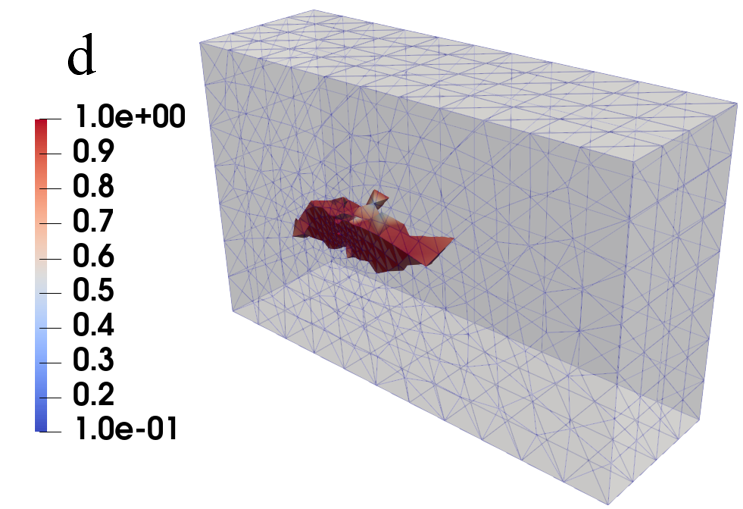
\includegraphics[scale=0.34]{6.25.png}
\caption{830 cycles}
\end{subfigure}
\begin{subfigure}{0.34\textwidth}
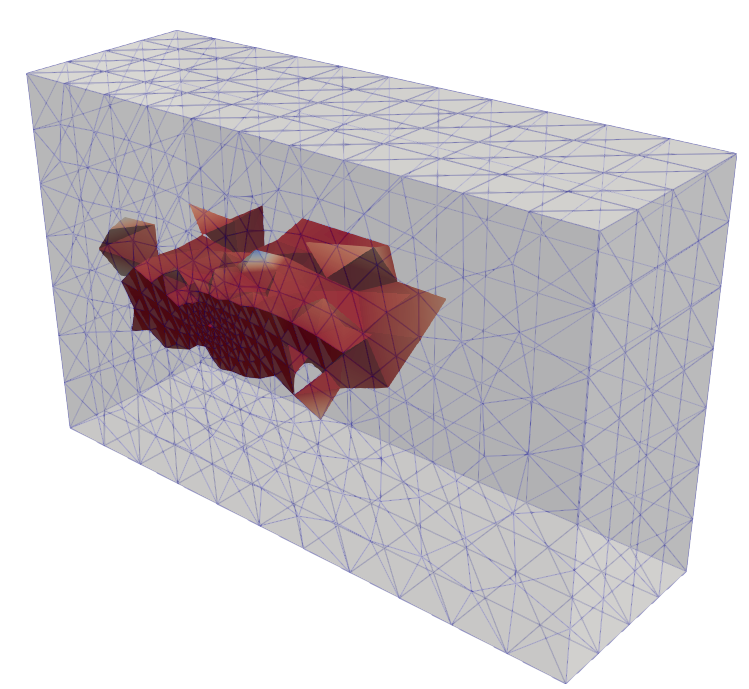
\includegraphics[scale=0.26, center]{8.25.png}
\caption{1025 cycles}
\end{subfigure}
\begin{subfigure}{0.27\textwidth}
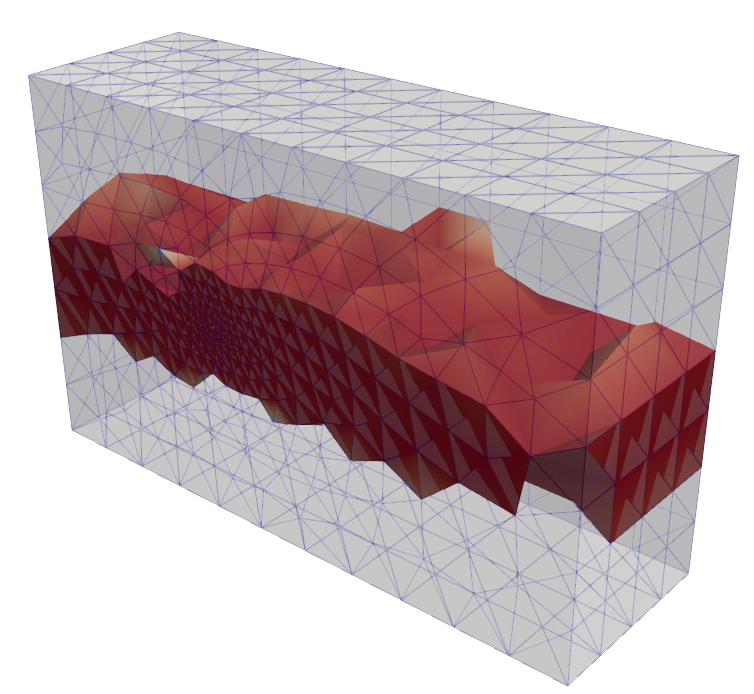
\includegraphics[scale=0.26, center]{12.35.png}
\caption{1725 cycles}
\end{subfigure}
\caption{Crack phase field $d$, nucleation and propagation through the 100 MPa loaded specimen simulation that includes a 0.1 mm pore at three different number of effective cycles.}
% /home/nicolo/projects/GreyCastIron_Raffaele/Simulations/Pore_01mm_dynamics.i
\label{damage field}
\end{figure}
\begin{figure} [ht]
\begin{subfigure}{0.5\textwidth}
\hspace{-8mm}
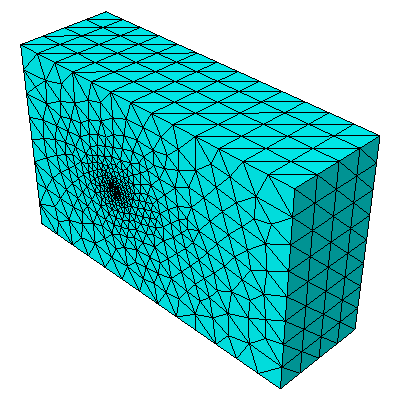
\includegraphics[scale=0.52, center]{graphite_mesh.png}
\vspace{20mm}
\caption{Mesh of the specimen with the graphite flake}
% path to file
\label{mesh graphite}
\end{subfigure}
\begin{subfigure}{0.5\textwidth}
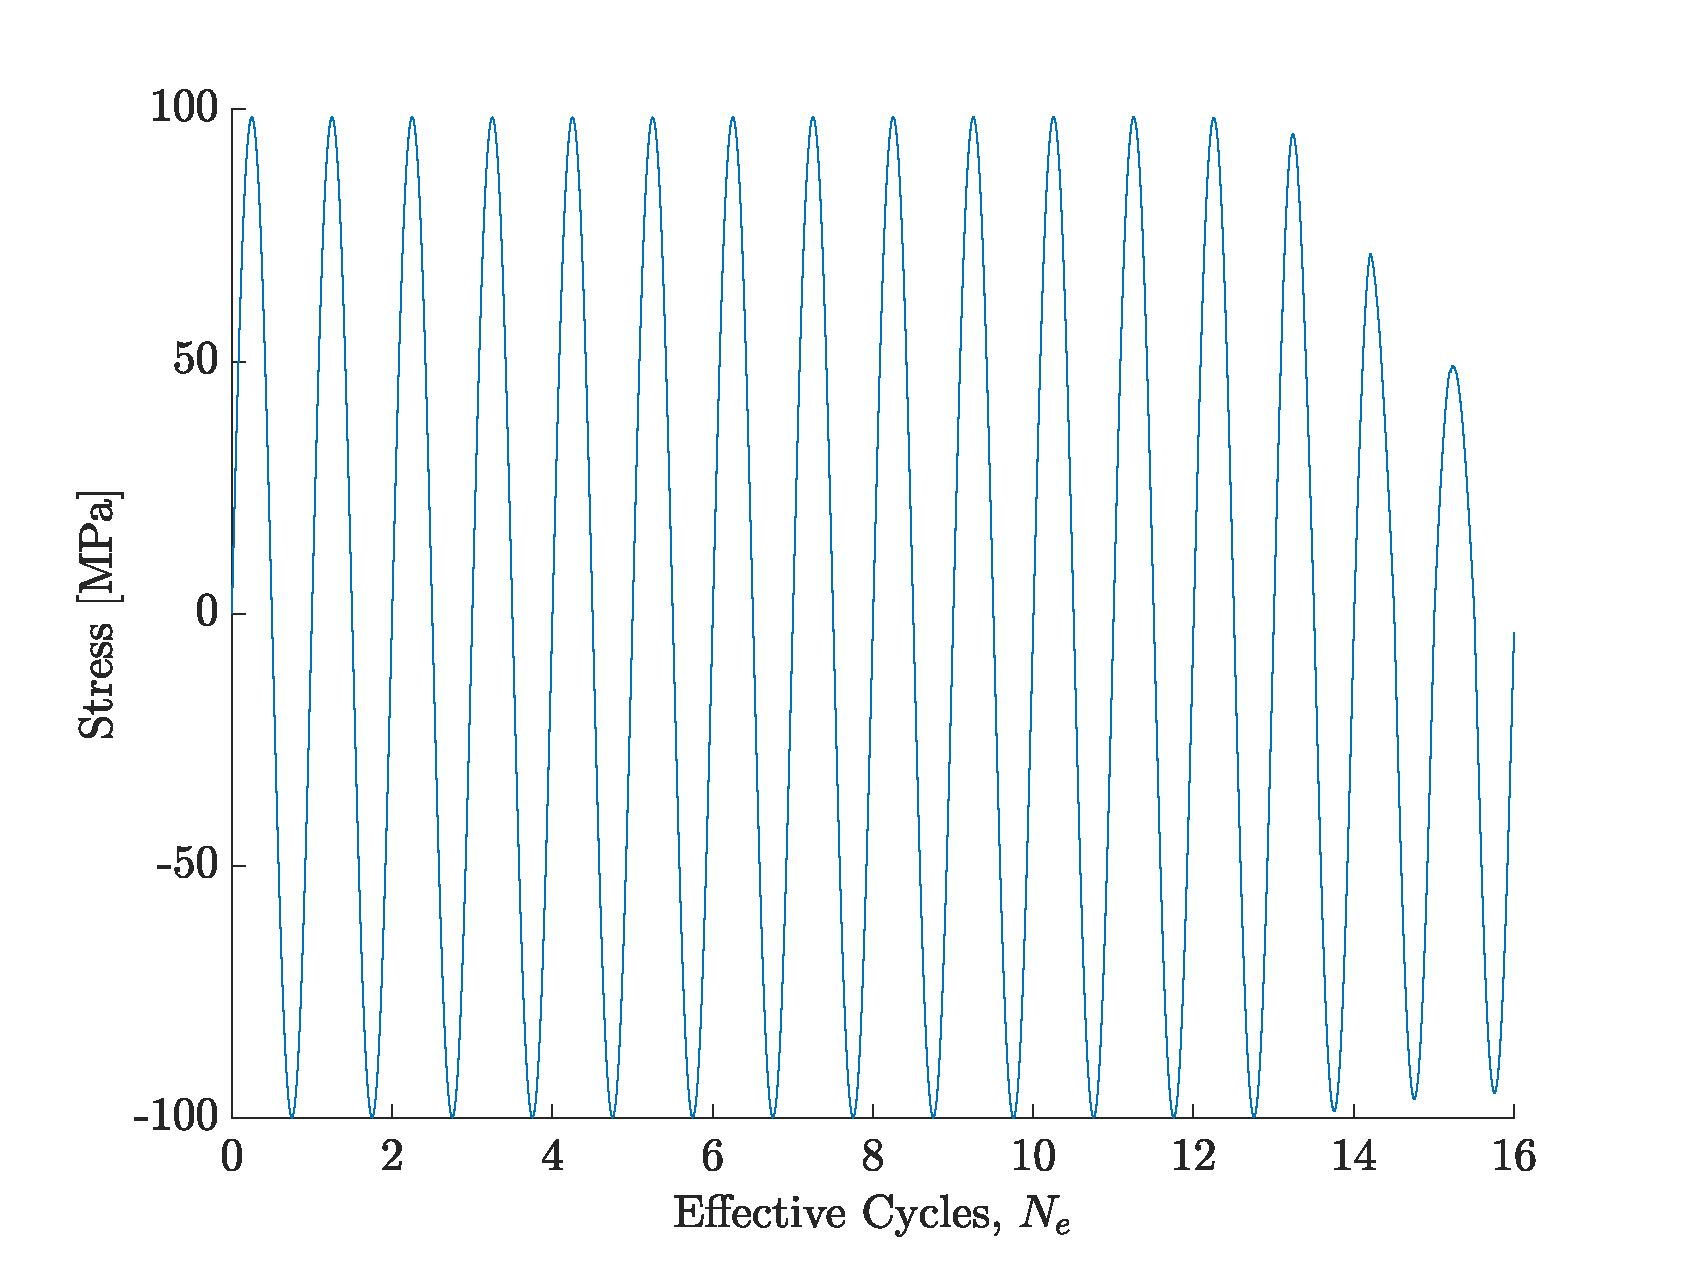
\includegraphics[scale=0.35, center]{alternating_graphite.eps}
\caption{Alternating average stress on the load surface}
\label{graphite alternating}
\end{subfigure}
\caption{Model with graphite.}
\end{figure}

\begin{figure} [ht]
\begin{subfigure}{0.51\textwidth}
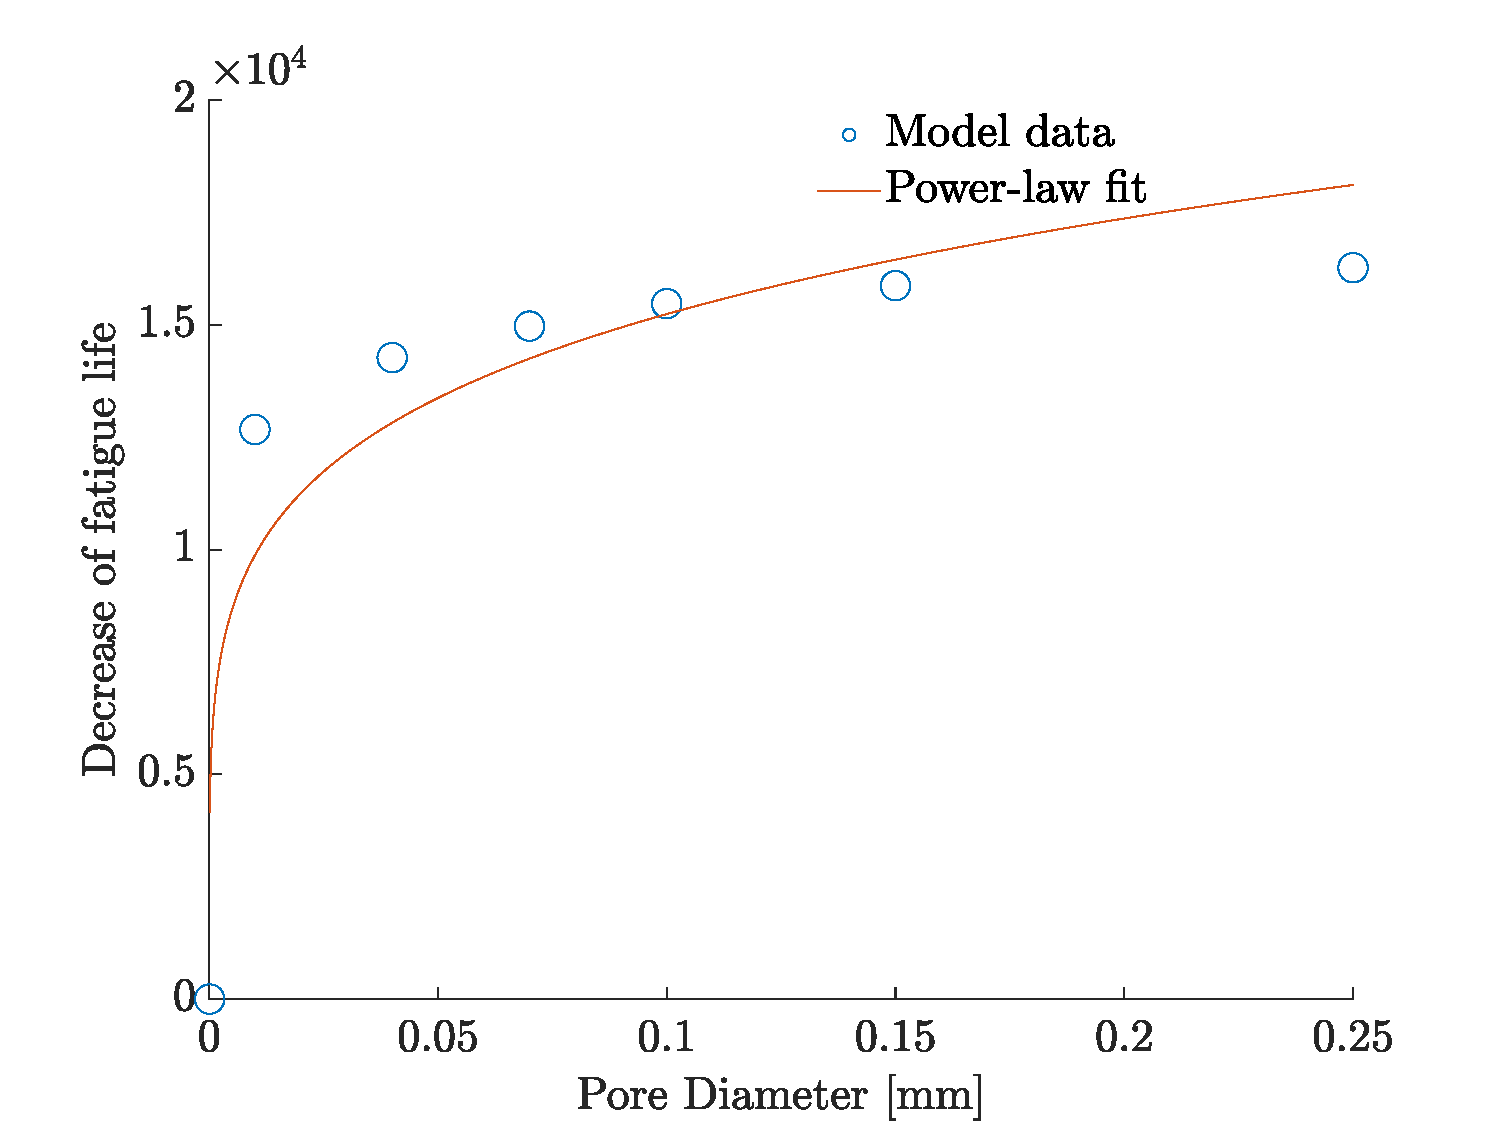
\includegraphics[scale=0.37, center]{reduction_pore.eps}
\caption{Porosity}
\label{reduction_porosity}
\end{subfigure}
\begin{subfigure}{0.55\textwidth}
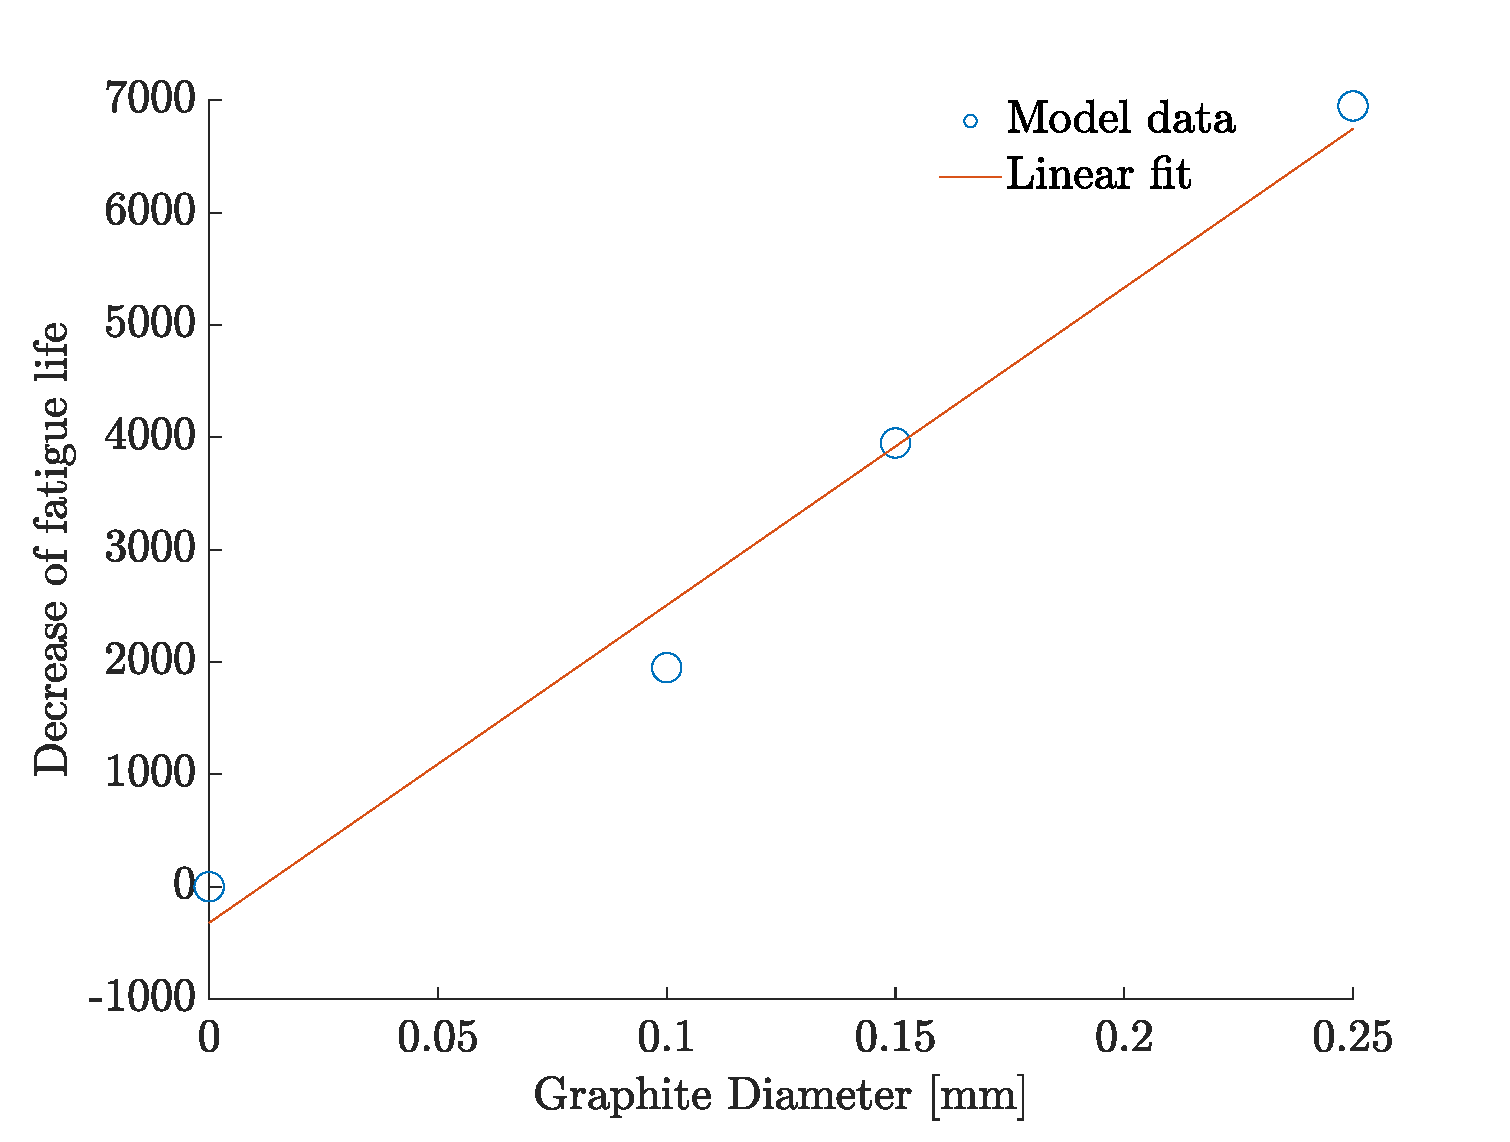
\includegraphics[scale=0.37, center]{decrease_graphite.eps}
\caption{Graphite flakes}
\end{subfigure}
\caption{Reduction of fatigue life of grey cast iron specimen.}
\label{reduction}
\end{figure}

\subsection{Analysis of model simulations with micro-structural features}
\label{analysis of features}
After the simulations has been performed, the analysis of the results are presented. Inspecting figures \ref{pore alternating} and \ref{graphite alternating}, it can be observed that the pore specimen fails after 1725 cycles and the specimen with the graphite flake after 15250 cycles. In addition, the range of pore sizes modelled, resulted in a fatigue life ranging from 4525-925 cycles, where as the range of graphite flake sizes modelled, from 15250-10250 cycles. The range of the fatigue life of the different pore sizes was compared with the experimental data from this work shown in figure \ref{S_N}. It could be seen that they are very closely related, as the three 100 MPa experimental specimens failed after 2500-7500 cycles. Also, if specifically assessing the 0.04 and 0.07 mm pore size models from figure \ref{reduction_porosity}, it can be seen that they failed after 2925 and 2225 cycles respectively. This can be considered as a direct match with the 2500 cycles of failure shown from the two out of the three 100 MPa experimental specimens. Moreover, the crack phase field $d$, from figure \ref{evolution}, shows that the crack will nucleate from the pore, to the full length and width of the specimen as soon as it fractures. In addition, when directly comparing the models with the 0.1 mm size pore and graphite flake, it is deduced that the effect of the pore is much higher (8 times) than the graphite flake on the fatigue life of the specimen. This is supported as well, as the specimens with the graphite flake have reached approximately 10 times more number of cycles than the pore ones. Lastly, the decrease of the fatigue life against the different pore and graphite flake sizes in figure \ref{reduction}, showed a power-law and a linear regression fit respectively. 

\section{Discussion}
The research problem investigated was focused on understanding how the microstructure, porosity, and graphite content affect the cyclic fatigue properties of grey cast iron and how to assess its lifespan. The main objective of the project includes to develop a multi-scale model that can accurately predict the lifetime of grey cast iron components at different length scales, accounting for micro-structural variations, and loading conditions.

\noindent The project's key findings are stated in section \ref{analysis of features}. As suggested, it shows that the simulations with the estimated pore size range from the optical microscopy images, match the experimental data of this work. This is crucial because it demonstrates that when a fractured specimen's surface is analyzed using image analysis to estimate a pore size, it is possible to determine its remaining lifespan. This observation completes the second part of objective \ref{O6}, where the model was used to reproduce the experimental results of this work. In addition, in figure \ref{damage field}, the crack phase field nucleates from the pore where the largest stress concentration is applied and evolves to its full length when it fractures.

\noindent Moreover, as it was shown from the results, when comparing the effect of the porosity with the graphite flake, it is clear that porosity has a much stronger negative effect on the fatigue life of the grey cast iron specimen. Consequently, combining the fact that porosity has a stronger negative effect than graphite on the fatigue life of grey cast iron, together with the pore specimen simulation that showed how the crack is nucleating from the pore, it can be evaluated that porosity is the main site for crack nucleation and propagation.

\noindent Furthermore, the reduction of the fatigue life of the specimen containing a pore or a graphite flake at different sizes is investigated. As mentioned before, a power-law and a linear relationship were established against the pore and graphite flake sizes respectively. This is very important as it means that estimations of the decrease of the fatigue life of the specimen, containing any graphite flake or pore size, can be deduced, accomplishing at the same time, objective \ref{O7}.

\noindent As the model was accurately matching the results of the literature and this project's experiments it can be deduced that the computational toolbox that can be used to asses the reduction of the fatigue life of specimens, as a function of porosity and graphite content was created, and hence objective \ref{O8} is achieved. This is because after incorporating the micro-structural features that was deduced in the image analysis into the model, it was able to accurately estimate the reduction of its fatigue life, and therefore its component that it was extracted from.

\noindent Upon reviewing the literature, it is evident that there is limited information available on grey cast iron. When the project is contextualized within the existing literature in the field, it becomes evident that it can play a crucial role in helping to advance our understanding of the topic. To start with, it was able to deduce a relationship between porosity and grey cast iron, which was not investigated in the past, as complex microscopy techniques were needed and were not available. However, it aligned with the previously researched materials where pore material specimens were fatigue tested and resulted again in a decrease of their fatigue life. Moreover, it was agreed with researched literature that porosity has a higher negative effect on the fatigue life of cast iron than graphite. In addition, the phase field fracture modelling was extended to account for the  cyclic loading brittle fracture, something that was done before but not with the same way.

\noindent In the context of the wider vision of the project it contributes a lot to the engineering and sustainability field. This is because a non-destructive technique was demonstrated, where with small sample analysis, and a computer model, it can be then carried out to the infrastructure components. This was demonstrated through this project where the stanchion part from the Clifton Suspension bridge was investigated by extracting a small sample.

\section{Limitations and future work}
Some limitations and the corresponding future work associated with them are explained below. Firstly, the project only considered the effect of fully reversed axial loading on the fatigue life of the material. Therefore, future studies could investigate the effect of other types of loading conditions such as bending and torsion. Moreover, the computational toolbox developed in this study could be improved and expanded to include more complex loading conditions and a wider range of materials. Future research could focus on the development of more advanced modelling techniques to improve the accuracy of fatigue life predictions. In addition, the study only considered the effects of pore and graphite content on the fatigue life of the specimens and did not investigate other factors that could affect the safety and remaining life of these structures, such as corrosion, impact damage, and environmental factors. Future work could include the investigation of these factors for a more accurate prediction.

\section{Conclusion}
The study aimed to investigate how microstructure, porosity, and graphite content impact the cyclic fatigue properties of grey cast iron and develop a multi-scale model to predict grey cast iron lifespan under different conditions. Through mechanical testing, optical and scanning electron microscopy, and the extension of the phase field fracture model to account for cyclic loading, the researched literature experimental results and the experimental results of this work, were reproduced. Through the work, it was established as well, that porosity has a much higher negative effect on the fatigue life of the grey cast iron specimens than graphite. The project has significant implications for the engineering and sustainability field as it demonstrated a non-destructive technique that can be applied to infrastructure components. Overall, the project highlights the potential of this approach to improve the method of assessing infrastructure components, while minimizing damage, improving safety, and promoting sustainability.

\cite{Cyclic}
\bibliographystyle{plain}
\bibliography{references}
\end{document} 